%* 
%* ------------------------------------------------------------------
%* UserManual.tex - Model Railroad System user documents
%* Created by Robert Heller on Sat Nov  9 15:33:35 2002
%* ------------------------------------------------------------------
%* Modification History: $Log$
%* Modification History: Revision 1.2  2007/05/06 12:49:41  heller
%* Modification History: Lock down  for 2.1.8 release candidate 1
%* Modification History:
%* Modification History: Revision 1.1  2002/11/09 21:21:07  heller
%* Modification History: Time Table User Manual
%* Modification History:
%* Modification History: Revision 1.1  2002/07/28 14:03:50  heller
%* Modification History: Add it copyright notice headers
%* Modification History:
%* ------------------------------------------------------------------
%* Contents:
%* ------------------------------------------------------------------
%*  
%*     Model RR System, Version 2
%*     Copyright (C) 1994,1995,2002  Robert Heller D/B/A Deepwoods Software
%* 			51 Locke Hill Road
%* 			Wendell, MA 01379-9728
%* 
%*     This program is free software; you can redistribute it and/or modify
%*     it under the terms of the GNU General Public License as published by
%*     the Free Software Foundation; either version 2 of the License, or
%*     (at your option) any later version.
%* 
%*     This program is distributed in the hope that it will be useful,
%*     but WITHOUT ANY WARRANTY; without even the implied warranty of
%*     MERCHANTABILITY or FITNESS FOR A PARTICULAR PURPOSE.  See the
%*     GNU General Public License for more details.
%* 
%*     You should have received a copy of the GNU General Public License
%*     along with this program; if not, write to the Free Software
%*     Foundation, Inc., 675 Mass Ave, Cambridge, MA 02139, USA.
%* 
%*  
%* 
\documentclass[12pt,notitlepage,twoside]{book}
\usepackage{graphicx}
\usepackage{mathptm}
\usepackage{times}
\usepackage{makeidx}
\usepackage{url}
\usepackage{supertabular}
\usepackage{MyTitlepage}
\usepackage{MyBibIndex}
\usepackage{listings}
\usepackage{tips}
\pagestyle{headings}
\makeindex
\emergencystretch=50pt
\begin{document}
\lstset{language=Tcl,basicstyle=\footnotesize,numbers=left,stepnumber=5}% Most examples will be in Tcl
\newcommand{\MRRSubTitle}{User Manual}
%* 
%* ------------------------------------------------------------------
%* titlepage.tex - Common documentation title page
%* Created by Robert Heller on Sun Oct 13 15:59:49 2002
%* ------------------------------------------------------------------
%* Modification History: $Log$
%* Modification History: Revision 1.3  2007/10/22 17:17:27  heller
%* Modification History: 10222007
%* Modification History:
%* Modification History: Revision 1.2  2004/04/14 23:20:24  heller
%* Modification History: Updated copyright.
%* Modification History:
%* Modification History: Revision 1.1  2002/10/17 00:02:24  heller
%* Modification History: Documentation support files.
%* Modification History:
%* Modification History: Revision 1.1  2002/07/28 14:03:50  heller
%* Modification History: Add it copyright notice headers
%* Modification History:
%* ------------------------------------------------------------------
%* Contents:
%* ------------------------------------------------------------------
%*  
%*     Model RR System, Version 2
%*     Copyright (C) 1994,1995,2002  Robert Heller D/B/A Deepwoods Software
%* 			51 Locke Hill Road
%* 			Wendell, MA 01379-9728
%* 
%*     This program is free software; you can redistribute it and/or modify
%*     it under the terms of the GNU General Public License as published by
%*     the Free Software Foundation; either version 2 of the License, or
%*     (at your option) any later version.
%* 
%*     This program is distributed in the hope that it will be useful,
%*     but WITHOUT ANY WARRANTY; without even the implied warranty of
%*     MERCHANTABILITY or FITNESS FOR A PARTICULAR PURPOSE.  See the
%*     GNU General Public License for more details.
%* 
%*     You should have received a copy of the GNU General Public License
%*     along with this program; if not, write to the Free Software
%*     Foundation, Inc., 675 Mass Ave, Cambridge, MA 02139, USA.
%* 
%*  
%* 
%* 
%* $Id$  
%* 

\title{Model Railroad System \\ A collection of utilities for Model Railroaders\\ \MRRSubTitle}
\author{Robert Heller \\ Deepwoods Software \\ Wendell, MA, USA}
\date{\today}
\begin{titlepage}

\maketitle

%\begin{centering}
%\epsfig{file=../Cover1.ps} \\
%\end{centering}

\clearpage


This documentation was prepared with \LaTeX.

This document describes version 2 of the Model Railroad System package.

\vspace{.25in}



{\small Copyright \copyright 1994,1995,2002-2012 by Robert Heller D/B/A Deepwoods
Software}

\vspace{.25in}

All rights reserved.  Permission is granted to copy this document in
electronic form only, so long as it is with the software it
documents. 

The author, Robert Heller, may be contacted electronically (E-Mail) via
the following:

\begin{description}
\item[FidoNet] 1:321/153, Locks Hill BBS.
\item[InterNet] heller@deepsoft.com
\end{description}

Web site URL: {\tt http://www.deepsoft.com/}.

\thispagestyle{empty}
\setcounter{page}{0}
\clearpage

\end{titlepage}


\pagenumbering{roman}
\tableofcontents
\listoffigures
\listoftables
\cleardoublepage
%       
%* 
%* ------------------------------------------------------------------
%* Preface.tex - Preface to the user manual
%* Created by Robert Heller on Sat Apr 21 10:32:44 2007
%* ------------------------------------------------------------------
%* Modification History: $Log$
%* Modification History: Revision 1.1  2007/05/06 12:49:40  heller
%* Modification History: Lock down  for 2.1.8 release candidate 1
%* Modification History:
%* Modification History: Revision 1.1  2002/07/28 14:03:50  heller
%* Modification History: Add it copyright notice headers
%* Modification History:
%* ------------------------------------------------------------------
%* Contents:
%* ------------------------------------------------------------------
%*  
%*     Model RR System, Version 2
%*     Copyright (C) 1994,1995,2002-2005  Robert Heller D/B/A Deepwoods Software
%* 			51 Locke Hill Road
%* 			Wendell, MA 01379-9728
%* 
%*     This program is free software; you can redistribute it and/or modify
%*     it under the terms of the GNU General Public License as published by
%*     the Free Software Foundation; either version 2 of the License, or
%*     (at your option) any later version.
%* 
%*     This program is distributed in the hope that it will be useful,
%*     but WITHOUT ANY WARRANTY; without even the implied warranty of
%*     MERCHANTABILITY or FITNESS FOR A PARTICULAR PURPOSE.  See the
%*     GNU General Public License for more details.
%* 
%*     You should have received a copy of the GNU General Public License
%*     along with this program; if not, write to the Free Software
%*     Foundation, Inc., 675 Mass Ave, Cambridge, MA 02139, USA.
%* 
%*  
%* 

\chapter*{Preface}
\markboth{PREFACE}{PREFACE}%
\addcontentsline{toc}{chapter}{Preface}
\label{chpt:Preface}
\typeout{$Id$}

This is the user manual for the Model Railroad system.  It is a ``work
in progress'' and I will be adding chapters as I write the various
self-contained ``main programs''.

%
\cleardoublepage
\pagenumbering{arabic}
%
%* 
%* ------------------------------------------------------------------
%* Introduction.tex - Introduction
%* Created by Robert Heller on Thu Apr 19 14:24:42 2007
%* ------------------------------------------------------------------
%* Modification History: $Log$
%* Modification History: Revision 1.1  2007/05/06 12:49:38  heller
%* Modification History: Lock down  for 2.1.8 release candidate 1
%* Modification History:
%* Modification History: Revision 1.1  2002/07/28 14:03:50  heller
%* Modification History: Add it copyright notice headers
%* Modification History:
%* ------------------------------------------------------------------
%* Contents:
%* ------------------------------------------------------------------
%*  
%*     Model RR System, Version 2
%*     Copyright (C) 1994,1995,2002-2005  Robert Heller D/B/A Deepwoods Software
%* 			51 Locke Hill Road
%* 			Wendell, MA 01379-9728
%* 
%*     This program is free software; you can redistribute it and/or modify
%*     it under the terms of the GNU General Public License as published by
%*     the Free Software Foundation; either version 2 of the License, or
%*     (at your option) any later version.
%* 
%*     This program is distributed in the hope that it will be useful,
%*     but WITHOUT ANY WARRANTY; without even the implied warranty of
%*     MERCHANTABILITY or FITNESS FOR A PARTICULAR PURPOSE.  See the
%*     GNU General Public License for more details.
%* 
%*     You should have received a copy of the GNU General Public License
%*     along with this program; if not, write to the Free Software
%*     Foundation, Inc., 675 Mass Ave, Cambridge, MA 02139, USA.
%* 
%*  
%* 

\chapter{Introduction}
\label{chapt:Introduction}
\typeout{$Id$}

This manual presents some information about how to write programs that
use various parts of Model Railroad System to control and manage various
aspects of operating your model railroad.  The Model Railroad System
includes code that interfaces with special hardware, including the PI
Engineering Raildriver Console (see
Chapter~\ref{chapt:RaildriverServer}), a Bruce Chubb network of control
nodes (see  Chapter~\ref{chapt:CMRIProgramming}), and a Lenz XPressNet
network (see Chapter~\ref{chapt:XPressNetProgramming}).  Also included
are a collection of Tcl scripts that implement a collection of widgets
that are useful for various aspects of programming utilities for a model
railroad system.

\part{Universal Test Program}
\label{part:univtest}
%* 
%* ------------------------------------------------------------------
%* UniversalTestReference.tex - Universal Test Program Reference Manual
%* Created by Robert Heller on Tue Aug  4 17:40:55 2009
%* ------------------------------------------------------------------
%* Modification History: $Log$
%* Modification History: Revision 1.1  2002/07/28 14:03:50  heller
%* Modification History: Add it copyright notice headers
%* Modification History:
%* ------------------------------------------------------------------
%* Contents:
%* ------------------------------------------------------------------
%*  
%*     Model RR System, Version 2
%*     Copyright (C) 1994,1995,2002-2005  Robert Heller D/B/A Deepwoods Software
%* 			51 Locke Hill Road
%* 			Wendell, MA 01379-9728
%* 
%*     This program is free software; you can redistribute it and/or modify
%*     it under the terms of the GNU General Public License as published by
%*     the Free Software Foundation; either version 2 of the License, or
%*     (at your option) any later version.
%* 
%*     This program is distributed in the hope that it will be useful,
%*     but WITHOUT ANY WARRANTY; without even the implied warranty of
%*     MERCHANTABILITY or FITNESS FOR A PARTICULAR PURPOSE.  See the
%*     GNU General Public License for more details.
%* 
%*     You should have received a copy of the GNU General Public License
%*     along with this program; if not, write to the Free Software
%*     Foundation, Inc., 675 Mass Ave, Cambridge, MA 02139, USA.
%* 
%*  
%* 
\chapter{Universal Test Program Reference}
\label{chpt:univtest:Reference}
\typeout{$Id$}

The Universal Test program is used to test the I/O ports on a USIC,
SUSIC, or SMINI node.  It is a port of the universal test program that
is shown in \cite{Chubb89} and \cite{Chubb03}.

\section{Main GUI Elements}

\subsection{Main Window}
\begin{figure}[hbpt]
\begin{centering}
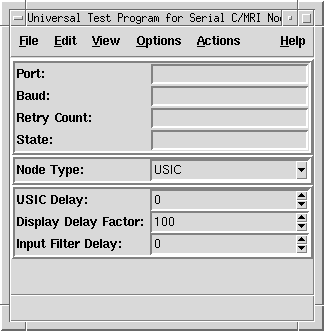
\includegraphics{UTMain.png}
\caption{The main window of the Universal Test Program}
\label{fig:ut:main}
\end{centering}
\end{figure}
The main window upon start up looks like Figure~\ref{fig:ut:main}. The
node type and initialization factors can be set.  The Display Delay
Factor is the number of hundredths of seconds between bit tests.  The
default value of 100 means a 1 second delay between output bits.  The
Input Filter Delay is the number of hundredths of seconds between bit
tests for the input port (wraparound) test.  The default value of 0
means to test as fast as possible (the program will stop if there is an
error).

\subsection{Open New Port}
\begin{figure}[hbpt]
\begin{centering}
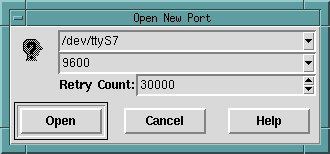
\includegraphics{UTNewCard.png}
\caption{The Open New Port dialog box of the Universal Test Program}
\label{fig:ut:new}
\end{centering}
\end{figure}
The New menu item on the File menu opens the serial port (/dev/ttySn)
the Chubb node is connected to and set the baud rate and retry count,
as shown in Figure~\ref{fig:ut:new}. The Open menu item on the File
menu opens the previously open port (if the port is currently open, it
is closed first).  The board at UA 0 is then initialized.  For USIC and
SUISC cards, it is presumed that the backplane contains just one output
card (in the first slot) for output testing, and one each output and
input card for the wraparound test (output card in the first slot and
the input card in the second slot).

\section{Tests}

There are two tests available: the output port test, which tests an output
port card and the wraparound test, which tests an input port card using
an output port card.  The output card test uses an output card LED test
plug in and lights up one LED at a time.  The wraparound uses the
wraparound cable to connect an input card to an output card and writes
bit values to the output card and reads these values on the input card
and compares what was written with what was read. These tests are
selected from the Actions menu.  

\subsection{Test Output Card}

\begin{figure}[hbpt]
\begin{centering}
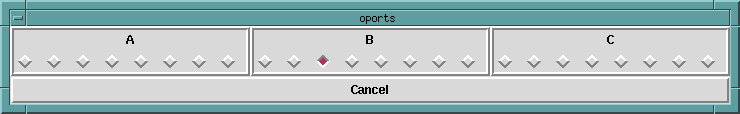
\includegraphics[width=5in]{UTOutputTest.png}
\caption{The Output Card Test Dialog Box}
\label{fig:ut:outtest}
\end{centering}
\end{figure}
The output card test displays the dialog box shown in
Figure~\ref{fig:ut:outtest}.  The lit up indicator on the dialog box
should match a corresponding LED on the output card LED test plug. The
test is repeated until canceled.

\subsection{Wraparound Test}

\begin{figure}[hbpt]
\begin{centering}
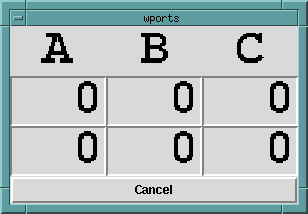
\includegraphics[width=5in]{UTWrapAround.png}
\caption{The Wraparound Test Dialog Box}
\label{fig:ut:wraptest}
\end{centering}
\end{figure}
The wraparound test displays the dialog box shown in
Figure~\ref{fig:ut:wraptest}.  The hexadecimal numbers represent the bit
pattern written to the output card.  These values are read back from the
input card and compared.  If there is a difference, the test stops and
displays the error bit pattern.




\part{Time Table (V2)}
\label{part:timetable}
%* 
%* ------------------------------------------------------------------
%* TTTutorial.tex - Time Table (V2) Tutorial
%* Created by Robert Heller on Thu Apr 26 12:32:29 2007
%* ------------------------------------------------------------------
%* Modification History: $Log$
%* Modification History: Revision 1.1  2007/05/06 12:49:40  heller
%* Modification History: Lock down  for 2.1.8 release candidate 1
%* Modification History:
%* Modification History: Revision 1.1  2002/07/28 14:03:50  heller
%* Modification History: Add it copyright notice headers
%* Modification History:
%* ------------------------------------------------------------------
%* Contents:
%* ------------------------------------------------------------------
%*  
%*     Model RR System, Version 2
%*     Copyright (C) 1994,1995,2002-2005  Robert Heller D/B/A Deepwoods Software
%* 			51 Locke Hill Road
%* 			Wendell, MA 01379-9728
%* 
%*     This program is free software; you can redistribute it and/or modify
%*     it under the terms of the GNU General Public License as published by
%*     the Free Software Foundation; either version 2 of the License, or
%*     (at your option) any later version.
%* 
%*     This program is distributed in the hope that it will be useful,
%*     but WITHOUT ANY WARRANTY; without even the implied warranty of
%*     MERCHANTABILITY or FITNESS FOR A PARTICULAR PURPOSE.  See the
%*     GNU General Public License for more details.
%* 
%*     You should have received a copy of the GNU General Public License
%*     along with this program; if not, write to the Free Software
%*     Foundation, Inc., 675 Mass Ave, Cambridge, MA 02139, USA.
%* 
%*  
%* 

\chapter{Time Table (V2) Tutorial}
\label{chpt:tt:Tutorial}
\typeout{$Id$}

\index{Time Table!Tutorial|(} The Time Table is a program designed to
create railroad employee timetables.  The program's main display is a
graph of time (of day) versus distance (along the railroad), gridded at
time intervals and at station stops.  Trains schedules are represented
as colored lines on this graph, with diagonals representing train
movement at speed and horizontal lines representing trains ``siting''
at stations (layovers or switching).

\section{Creating a new time table}

To create an new time table select the \verb=File->New= menu item or
the 
\includegraphics{TTNewTool.png} toolbar button. A ``Create a New
Time Table'' dialog, described in
Section~\ref{sect:tt:createnewtimetable}. is displayed.  This dialog
box collects three pieces of information: the name of the new time
table, the total time (in minutes) the time table will cover (there are
1440 minutes in a 24 hour day), and the tick interval in minutes.  A
new time table can also me created from the command line by including
the options \verb=-totaltime= and \verb=-timeincrement= along with a
name for the new time table.

\subsection{Creating stations}

Once the name and the two time elements have been selected, a set of at
least two stations need to be created.  This is done with the ``Create
All Stations Dialog'',  described in
Section~\ref{sect:tt:CreateAllStationsDialog}.  This dialog box is
used to create stations, which can have zero or more storage tracks. 
Storage tracks are used when a train has a long layover (and needs to
be ``out of the way'' of other traffic) or when a train terminates and
the train set is re-used for a different schedule, generally in the
opposite direction. As the stations and their storage tracks are
created, they are displayed in the station listing in the upper part of
the dialog. 

\subsection{Creating cabs}

After creating all of the stations, zero or more cabs can be created. 
Cabs are mostly for switched block DC layouts, but creating ``cabs''
for a DCC layout is useful, since it allows for a way to visually group
trains operationally. Think of the cabs as a way of defining ``crews''
(operators).  This allows for things like crew (operator) changes as
the train moves to different parts of the layout for example.

\section{Creating trains}

Once the stations and cabs have been created, the program displays an
empty chart.  The chart's \verb=x= axis is time (in minutes).  The upper
section of the chart has the cabs (if any), the middle part of the chart
has the stations, and the bottom part of the chart has the storage
tracks (if any).  Now we can create a train.  This is done by selecting
either the \verb=Trains->Add Train= menu item, clicking on the add train
(
\includegraphics{TTaddtrain.png}) toolbar button or the 
\verb=Add a new train= button.  All of these display the ``Create New
Train Dialog'', described in Section~\ref{sect:tt:CreateNewTrainDialog}.

Trains have a (common) name, a number (or symbol), a class number, an average
speed, a scheduled departure time, and travel between two stations.  The
train's number (or symbol) needs to be a unique identification of the
train. The class is a whole number, with smaller numbers generally being
the ``higher'' class.  The class is used to indicate a train's priority
and is also used to group similar trains together.  The speed is the
(scale) speed the train will be traveling between stops.  The scheduled
departure time is the time the train is scheduled to leave its origin
station.  The origin and termination stations are the station end points
the train travels between.  The train will get a ``stop'' at every
intermediate station between these two stations.  Note that the train
won't be expected to actually stop at any station where the layover time
is set to zero.  Such stops would just be timekeeping points.

Once the train's basic information is set, the \verb=Schedule= button can be
clicked.  This shifts to the schedule page, where layovers and cab
assignments cab be set.  The \verb=Update= buttons propagate the
cab settings and adjust the times to allow for the layovers.  If the
train makes use of station storage tracks, the \verb=Storage= button can
be clicked and storage tracks selected.  When the train is fully
configured, the \verb=Done= button can be clicked to actually create the
train.

\section{Printing a time table}

Once all of the trains have been added, it it possible to ``print'' a
timetable.  The LaTeX system is used to format the time table and the
TimeTable program generates a \LaTeX{} source file (\verb=.tex=) and will
run the \LaTeX{} program, \verb=pdflatex=, to create a PDF file from the
\LaTeX{} source file.  This process is started with the
\verb=File->Print...= menu item or the
\includegraphics{TTprintTool.png} toolbar button.  This pops up the
``Print Dialog'', described in Section~\ref{sect:tt:PrintTimetableDialog}.
This dialog collects the name of the \LaTeX{} source file, and the path to the
\LaTeX{} processing programing, as well as a few other options.  It also
has a button to configure how the timetable will be formatted.  

The \verb=Configure= button pops up the ``Print Configuration Dialog'',
described in Section~\ref{sect:tt:PrintConfigurationDialog}, which has
three sections, a \verb=General= section which gets some general
configuration settings, a \verb=Multi= section for various
configuration settings relating to printing multiple tables, and a
\verb=Groups= section, for configuring groups of trains.  Some of the
configuration assumes some knowledge of \LaTeX. A visit to the \TeX{} and
\LaTeX{} web pages (\url{http://www.tug.org}) is a good place to start,
with the beginner's page at \url{http://www.tug.org/begin.html} as the
obvious starting point.  You don't really have to learn how to use
\LaTeX{}, you just need to have a \TeX/\LaTeX{} system installed.  The only
other issue is the \verb=TimeTable.sty= file.  This file either needs to be
installed somewhere in the \TeX/\LaTeX{} search path or it needs to be in
the same directory as the \LaTeX{} source file generated by the TimeTable
program. You will need to learn a little about \LaTeX{} if you want to
include various sorts of customizations.
\index{Time Table!Tutorial|)} 

%* 
%* ------------------------------------------------------------------
%* TTReference.tex - Time Table (V2) Reference
%* Created by Robert Heller on Thu Apr 26 12:33:54 2007
%* ------------------------------------------------------------------
%* Modification History: $Log$
%* Modification History: Revision 1.1  2007/05/06 12:49:40  heller
%* Modification History: Lock down  for 2.1.8 release candidate 1
%* Modification History:
%* Modification History: Revision 1.1  2002/07/28 14:03:50  heller
%* Modification History: Add it copyright notice headers
%* Modification History:
%* ------------------------------------------------------------------
%* Contents:
%* ------------------------------------------------------------------
%*  
%*     Model RR System, Version 2
%*     Copyright (C) 1994,1995,2002-2005  Robert Heller D/B/A Deepwoods Software
%* 			51 Locke Hill Road
%* 			Wendell, MA 01379-9728
%* 
%*     This program is free software; you can redistribute it and/or modify
%*     it under the terms of the GNU General Public License as published by
%*     the Free Software Foundation; either version 2 of the License, or
%*     (at your option) any later version.
%* 
%*     This program is distributed in the hope that it will be useful,
%*     but WITHOUT ANY WARRANTY; without even the implied warranty of
%*     MERCHANTABILITY or FITNESS FOR A PARTICULAR PURPOSE.  See the
%*     GNU General Public License for more details.
%* 
%*     You should have received a copy of the GNU General Public License
%*     along with this program; if not, write to the Free Software
%*     Foundation, Inc., 675 Mass Ave, Cambridge, MA 02139, USA.
%* 
%*  
%* 

\chapter{Time Table (V2) Reference}
\label{chpt:tt:Reference}
\typeout{$Id$}

The Time Table (V2) program is a hybrid program, consisting of a Tcl/Tk
GUI on top of a C++ class library.  The GUI provides the user interface
to the algorithms and data structures contained in the C++ class
library.  This program was inspired by chapter 8 of the book {\it How
to Operate Your Model Railroad}\cite{Chubb77} by Bruce A. Chubb.  I
strongly recommend reading this chapter fully before using this
program.  This program implements the methods described in this
chapter, in an automated fashion.

\section{Command Line Usage}

\begin{figure}[hbpt] 
\begin{centering} 
{\footnotesize
\begin{verbatim} 
TimeTable oldtimetablefile 
TimeTable -totaltime time -timeincrement time nameoftimetable 
\end{verbatim} 
}
\caption{Command Line Format for the TimeTable command} 
\label{fig:tt:cliusage} 
\end{centering} 
\end{figure}
There are two formats for the TimeTable program's command line.  The
command line can either have a single file name, the name of an
existing time table file or it can have two options (\texttt{-totaltime}
and \texttt{-timeincrement}) and the name of a new time table.  The first
form loads an existing time table (see
Section~\ref{sect:tt:loadexistingtimetable} and the second form creates
a new time table (see Section~\ref{sect:tt:createnewtimetable}.  These
two command line formats are shown in Figure~\ref{fig:tt:cliusage}. 

\section{Layout of the Main GUI}

\begin{figure}[hbpt]
\begin{centering}
\includegraphics[width=5in]{TTMainGUIBlank.png}
\caption{The main GUI screen of the Time Table (V2) Program}
\label{fig:tt:MainGUIBlank}
\end{centering}
\end{figure}
\begin{figure}[hbpt]
\begin{centering}
\includegraphics[width=5in]{TTMainGUIToolBar.png}
\caption{The Toolbar of the Time Table (V2) Program}
\label{fig:tt:MainGUIToolBar}
\end{centering}
\end{figure}
\begin{figure}[hbpt]
\begin{centering}
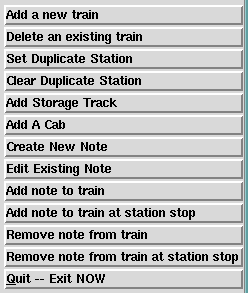
\includegraphics{TTMainGUIButtonMenu.png}
\caption{The Button Menu of the Time Table (V2) Program}
\label{fig:tt:MainGUIButtonMenu}
\end{centering}
\end{figure}
The main GUI window\index{Time Table!main GUI}, show in
Figure~\ref{fig:tt:MainGUIBlank}, contains a menu bar, a toolbar
(Figure~\ref{fig:tt:MainGUIToolBar}), a time table chart, and a button
menu (Figure~\ref{fig:tt:MainGUIButtonMenu}).

\section{Creating a New Time Table}
\label{sect:tt:createnewtimetable}

\begin{figure}[hbpt]
\begin{centering}
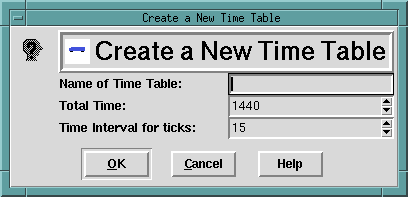
\includegraphics{TTCreateNewTT.png}
\caption{Create A New Time Table dialog}
\label{fig:tt:GetNewTimeTableDialog}
\end{centering}
\end{figure}
Creating a new time table can be done from the command line by
specifying a total time (in minutes) value with the \texttt{-totaltime}
option and a time increment value (in minutes) value with the
\texttt{-timeincrement} option and a name for the new time table (as
shown in the second line of Figure~\ref{fig:tt:cliusage}).  A new time
table can also be created with the \texttt{New} menu item of the
\texttt{File} menu or the

\includegraphics{TTNewTool.png} toolbar button. These later two methods
use the ``Create a New Time Table'' dialog, shown in
Figure~\ref{fig:tt:GetNewTimeTableDialog} to get the total time, time
increment, and the name of the new time table.  If there is a time
table file already loaded, a confirmation dialog will be displayed.

\subsection{Creating the station stops for a new time table}
\label{sect:tt:CreateAllStationsDialog}

\begin{figure}[hbpt]
\begin{centering}
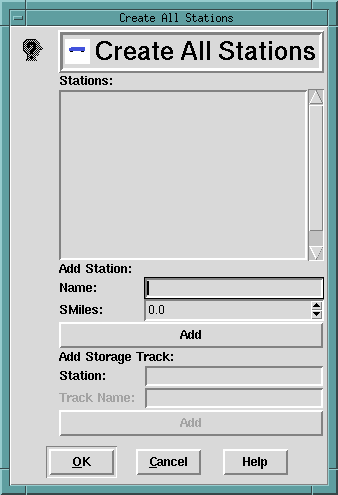
\includegraphics{TTCreateAllStations.png}
\caption{Create All Stations Dialog}
\label{fig:tt:CreateAllStationsDialog}
\end{centering}
\end{figure}
Stations for a time table must all be created when the time table is
created.  Stations cannot be added or removed later.  When a new time
table is created the ``Create All Stations Dialog'',  shown in
Figure~\ref{fig:tt:CreateAllStationsDialog} is displayed to create all
of the station stops.

\subsection{Creating an initial set of ``cabs''}

\begin{figure}[hbpt]
\begin{centering}
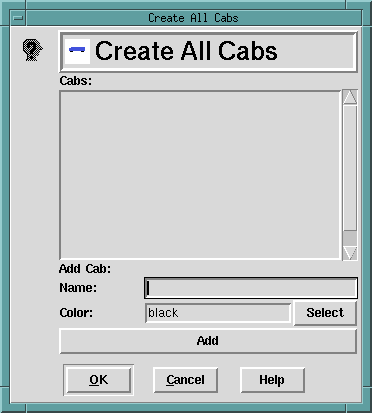
\includegraphics{TTCreateAllCabs.png}
\caption{Create All Cabs Dialog}
\label{fig:tt:CreateAllCabsDialog}
\end{centering}
\end{figure}
Once the stations have been created, an initial set of ``cabs'' can be
created.  Commonly, cabs are only used on block switch DC layouts, but
the cabs can be used as with a  DCC layout as a way to associate trains
with different operating ``crews'' (operators) or just to identify
different classes of trains by color, etc.  The ``Create All Cabs''
dialog, shown in Figure~\ref{fig:tt:CreateAllCabsDialog}, is used to
bulk create an initial set of cabs.

\begin{figure}[hbpt]
\begin{centering}   
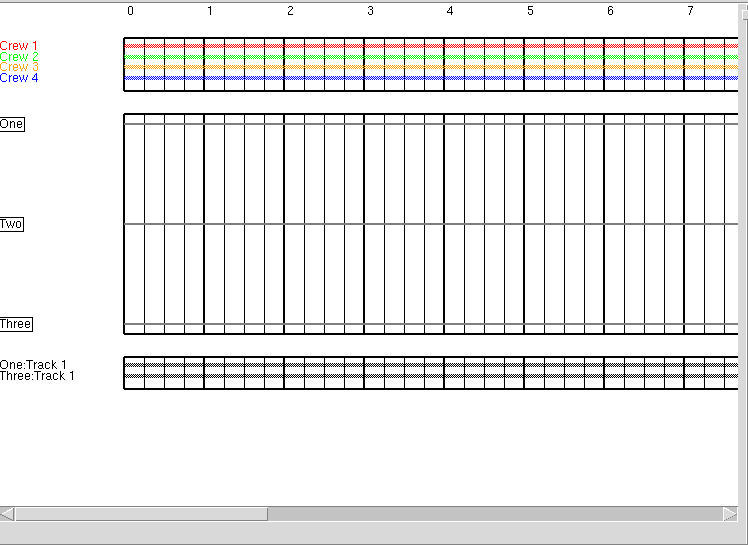
\includegraphics[width=5in]{TTChart3station.png}
\caption{Simple chart with three stations, four cabs, and two storage
tracks}
\label{fig:tt:Chart3station}
\end{centering}
\end{figure}   
A simple chart with three stations, four cabs (labeled ``Crew 1''
through ``Crew 4''), and two storage tracks is shown in
Figure~\ref{fig:tt:Chart3station}. 

\section{Loading an Exiting Time Table File}
\label{sect:tt:loadexistingtimetable}

An existing time table file can be loaded from the command line (as
shown in the first line of Figure~\ref{fig:tt:cliusage}),  with the
\texttt{Open...} menu item of the \texttt{File} menu or the

\includegraphics{TTOpenTool.png} toolbar button. If there is a time
table file already loaded, a confirmation dialog will be displayed.

\section{Saving a Time Table File}

The currently loaded time table can be saved with either the
\texttt{Save} (or \texttt{Save As...}) menu item of the \texttt{File} menu or
the \includegraphics{TTSaveTool.png} toolbar button. 

\section{Adding Trains}

Trains are added using the either the \texttt{Add Train} menu item of the
\texttt{Trains} menu, clicking on the add train
(
\includegraphics{TTaddtrain.png}) toolbar button or the \texttt{Add a
new train} button. All of these display the ``Create New Train
Dialog'', described in Section~\ref{sect:tt:CreateNewTrainDialog}.

\subsection{Create New Train Dialog}
\label{sect:tt:CreateNewTrainDialog}

\begin{figure}[hbpt]
\begin{centering}   
\includegraphics{TTCreateNewTrain1.png}
\caption{Creating a new train dialog, basic information}
\label{fig:tt:CreateNewTrain1}
\end{centering}
\end{figure}
The ``Create New Train Dialog'' first collects some basic information
about the new train, as shown in Figure~\ref{fig:tt:CreateNewTrain1}.
The basic train information consists of the train's common name, its
number (or symbol), its class number, its average speed, its scheduled
departure time, and the two stations it travels between.

The train's number (or symbol) needs to be a unique identification of
the train.  The common name need not be unique.  The class is a whole
number, with smaller numbers generally being the ``higher'' class. The
class is used to indicate a train's priority and is also used to group
similar trains together.  The speed is the (scale) speed the train will
be traveling between stops.  The scheduled departure time is the time
the train is scheduled to leave its origin station.  The origin and
termination stations are the station end points the train travels between.

\begin{figure}[hbpt]
\begin{centering}   
\includegraphics[width=5in]{TTCreateNewTrain2.png}
\caption{Creating a new train dialog, scheduling information}
\label{fig:tt:CreateNewTrain2}
\end{centering}
\end{figure}
The \texttt{Schedule} button selects the scheduling page of the ``Create a
New Train Dialog'', as shown in Figure~\ref{fig:tt:CreateNewTrain2}.  On
this page, the cab can be selected and layover periods at intermediate
stations can be set.  The \texttt{Update} buttons propagate the cab
settings and adjust the times to allow for the layovers.

\begin{figure}[hbpt]
\begin{centering}   
\includegraphics{TTCreateNewTrain3.png}
\caption{Creating a new train dialog, storage track selection}
\label{fig:tt:CreateNewTrain3}
\end{centering}
\end{figure}
The \texttt{Storage} button selects the storage track allocation page of
the ``Create a New Train Dialog'', as shown in
Figure~\ref{fig:tt:CreateNewTrain3}.  This page lists those stations
that have storage tracks available.  It only makes sense to select
storage tracks for intermediate stops if there is a layover or for
originating or terminating stops.

\section{Deleting Trains}
\label{sect:tt:DeletingTrains}

Trains are deleted using the \texttt{Delete Train} menu item of the
\texttt{Trains} menu, clicking on the delete train
(
\includegraphics{TTdeletetrain.png}) toolbar button or the
\texttt{Delete an Existing train} button. All of these display the
``Select One Train Dialog'', described in
Section~\ref{sect:tt:SelectOneTrainDialog}. A delete confirmation
dialog will also be displayed.

\section{Linking and Unlinking Duplicate Stations}

Duplicate stations occur mostly with ``out and back'' type layouts
where the opposite ends of the line are modeled with the same trackage
(usually a yard).  Duplicate stations also occur with reverse loops. In
all cases, these are stations which are logically different, but which
use the same tracks. There is an example in Figure~8-4 on page 86 of
\cite{Chubb77}. It is necessary to keep track of this trackage in the
schedule.  The duplicate station linking handles this. Duplicate
stations need to be setup before trains have been added.

The \texttt{Set Duplicate Station} and 
\texttt{Clear Duplicate Station} menu items of the \texttt{Stations} menu, the
\includegraphics{TTsetdupstation.png} and

\includegraphics{TTcleardupstation.png} toolbar buttons, and the
\texttt{Set Duplicate Station} and \texttt{Clear Duplicate Station} buttons
set and clear duplicate stations.

\section{Adding Station Storage Tracks}

Storage tracks are sidings where whole trains can be stored, either
during a long layover or between trips. The  \texttt{Add Storage Track}
menu item of the \texttt{Stations} menu, the

\includegraphics{TTaddstorage.png} toolbar button, or the  \texttt{Add
Storage Track} button are used to add a storage track to a station.

\section{Adding Cabs}

Generally ``Cabs'' refer to the separate throttle controls on a block
switched DC layout.  They are generally non-existent with a DCC layout,
but virtual cabs might be used as a way of assigning crews (operators)
to a train or to a segment of a train's run.  Cabs are added with the
\texttt{Add A Cab} menu item of the \texttt{Cabs} menu, the

\includegraphics{TTaddcab.png} toolbar button or the \texttt{Add A Cab}
button.

\section{Handling Notes}

Notes are brief memos about the operating rules in effect.  There is a
single pool of notes.  Notes from this pool can be associated either
with a whole train or with a train at a station stop.  The notes can
specify schedule exceptions (eg ``Daily except Saturdays, Sundays, and
Holidays''), or operating rules relating to meets.

\subsection{Creating New Notes and Editing Existing Notes}

\begin{figure}[hbpt]
\begin{centering}   
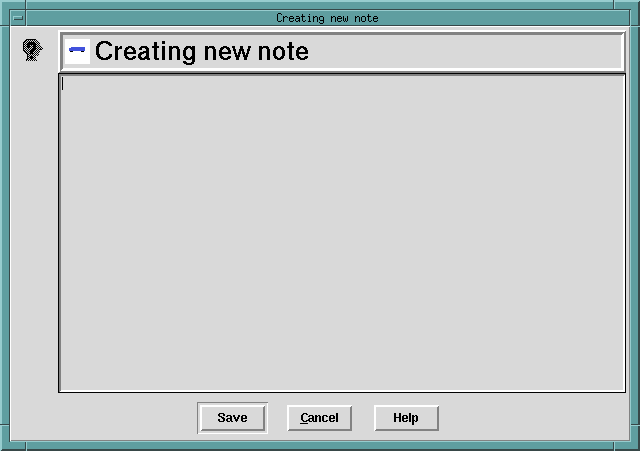
\includegraphics[width=5in]{TTEditNote.png}
\caption{Note editor dialog}
\label{fig:tt:EditNote}
\end{centering}
\end{figure}
Notes are created and edited the \texttt{Create New Note} and
\texttt{Edit Existing Note} menu items of the \texttt{Notes} menu, the

\includegraphics{TTcreatenote.png} and \includegraphics{TTeditnote.png}
toolbar buttons, or the \texttt{Create New Note} and 
\texttt{Edit Existing Note} buttons.  The the ``Note editor dialog'', shown in
Figure~\ref{fig:tt:EditNote} is used to create or edit the note.  Notes are
numbered consecutively starting with 1.

\subsection{Adding and Removing a Notes To Trains}

\begin{figure}[hbpt]
\begin{centering}
\includegraphics{TTAddNote.png}
\caption{Add (or Remove) Note dialog}
\label{fig:tt:AddNote}
\end{centering}
\end{figure}
Notes are added to trains or removed from trains with \texttt{Notes} menu
items \texttt{Add note to train}, \texttt{Add note to train at station stop},
\texttt{Remove note from train}, and 
\texttt{Remove note from train at station stop}; the
\includegraphics{TTaddnotetotrain.png},
\includegraphics{TTaddnotetotrainatstation.png},
\includegraphics{TTremovenotefromtrain.png}, and

\includegraphics{TTremovenotefromtrainatstation.png}; or the  
\texttt{Add note to train}, \texttt{Add note to train at station stop}, 
\texttt{Remove note from train}, and 
\texttt{Remove note from train at station stop} buttons.  All of these
display the ``Add (or Remove) Note dialog'', shown in
Figure~\ref{fig:tt:AddNote}.

\section{Printing a Time Table}

``Printing'' a time table actually means creating a \LaTeX{} file and
then processing that \LaTeX{} file through a \LaTeX{} processing program
(typically \texttt{pdflatex}).  \LaTeX{} provides the means to produce a
professionally formatted document and has the means to provide things
like table of contents and the creation of a final document in a
selection of different final formats, including PDF (via
\texttt{pdflatex}), PostScript (via \texttt{latex} and \texttt{dvips})
or HTML (via the \texttt{htlatex} script from \textit{tex4ht} package).

Much of the formatting is customizable through the insertion of \LaTeX{}
code fragments as well as through various parameter settings.  It is
also possible to edit the \LaTeX{} style file that comes with the Time
Table program (\texttt{TimeTable.sty}) to tweak some of the fine details
of the formatting as well\footnote{Some knowledge of how \LaTeX{} works
is recommended when messing with the style file.}.

The \texttt{Print} menu item of the \texttt{File} menu or the
\includegraphics{TTprintTool.png} toolbar button initiate the print
process by displaying the ``Print Timetable'' dialog, described in
Section~\ref{sect:tt:PrintTimetableDialog}.


\subsection{Print Timetable Dialog}
\label{sect:tt:PrintTimetableDialog}

\begin{figure}[hbpt]
\begin{centering}
\includegraphics[width=5in]{TTPrintTimetableDialog.png}
\caption{Print Timetable dialog}  
\label{fig:tt:PrintTimetableDialog}
\end{centering}
\end{figure}
The ``Print Timetable'' dialog, shown in
Figure~\ref{fig:tt:PrintTimetableDialog}, collects the basic
information needed to generate and process a \LaTeX{} source file from
the time table data structure.  This information consists of the name of
the name of the \LaTeX{} source file to create, the \LaTeX{} processing
program (\texttt{pdflatex} by default), whether to run the \LaTeX{}
processing three times (to get the table of contents right), the name of
any post processing command (such as \texttt{dvips} if using plain
\texttt{latex}).  Most of the time, this is enough for a standard, basic
time table.  The \texttt{Configure} button can be used to configure a
selection of options using a ``Print Configuration'' dialog, described
in Section~\ref{sect:tt:PrintConfigurationDialog}.

Once the settings and configuration have been set, the \texttt{Print}
initiates the process.  First a \LaTeX{} source file is generated, then
the \LaTeX{} processing program is run once or three times.  The output
from these runs are displayed in a process log window (\LaTeX{} outputs
a fair amount of diagnostic output, most of which can be ignored).  If
you are using the default processor (\texttt{pdflatex}), you should now
have a PDF file which can be viewed or printed with the PDF viewer of
your choice.

\subsection{Print Configuration Dialog}
\label{sect:tt:PrintConfigurationDialog}

\begin{figure}[hbpt]
\begin{centering}
\includegraphics[width=5in]{TTPrintConfigurationDialog1.png}
\caption{Print Configuration dialog, General settings}
\label{fig:tt:PrintConfigurationDialog1}
\end{centering}
\end{figure}
\begin{figure}[hbpt]
\begin{centering}
\includegraphics[width=5in]{TTPrintConfigurationDialog2.png}
\caption{Print Configuration dialog, Multi settings}
\label{fig:tt:PrintConfigurationDialog2}
\end{centering}
\end{figure}
\begin{figure}[hbpt]
\begin{centering}
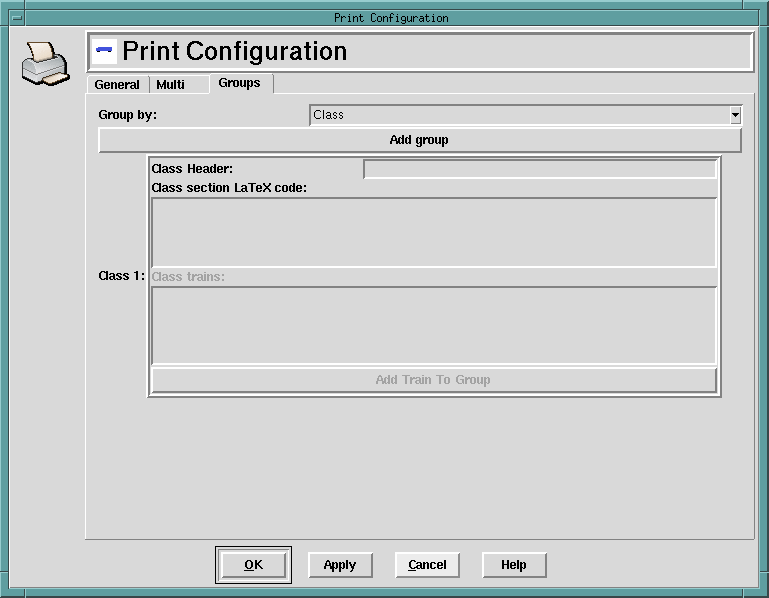
\includegraphics[width=5in]{TTPrintConfigurationDialog3.png}
\caption{Print Configuration dialog, Groups settings}
\label{fig:tt:PrintConfigurationDialog3}
\end{centering}
\end{figure}
The Print Configuration Dialog, shown in
Figures~\ref{fig:tt:PrintConfigurationDialog1};
\ref{fig:tt:PrintConfigurationDialog2}; and
\ref{fig:tt:PrintConfigurationDialog3}, provide for the setting of many
print configuration options. The general settings
(Figure~\ref{fig:tt:PrintConfigurationDialog1}), provide for setting the
title, subtitle, the date, whether to have \LaTeX{} format for double
sided printing, setting the time format, setting the logical direction
of trains, column widths, and including additional commands in the
\LaTeX{} preamble (usually including additional style
packages\footnote{The style pages supertabular and graphicx are already
included.} and style settings). The multi-table settings
(Figure~\ref{fig:tt:PrintConfigurationDialog2}), provide for settings
relating to time tables using multiple tables.  These settings include
whether to create a table of contents, whether to use multiple tables at
all, \LaTeX{} code to precede the table of contents, \LaTeX{} code to
precede notes section, the header to use if a single ``All Trains''
table is generated, and \LaTeX{} code to precede this single ``All
Trains'' table.  The groups settings
(Figure~\ref{fig:tt:PrintConfigurationDialog3}), provide for settings
for each group.  This includes whether to group by class or to manually
group trains and provides for setting the class or group heading and for
\LaTeX{} code to precede the group table, and if grouping manually,
selecting the trains in the group.

\section{Exiting From the Program}

The \texttt{Exit} (or \texttt{Close}) menu item of the \texttt{File}
menu, the 
\includegraphics{TTCloseTool.png} toolbar button, or the
\texttt{Quit -- Exit NOW} button exit the program.  A confirmation
dialog is displayed to get confirmation.

\section{Select One Train Dialog}
\label{sect:tt:SelectOneTrainDialog}

\begin{figure}[hbpt] 
\begin{centering}
\includegraphics{TTSelectOneTrain.png} 
\caption{Select One Train dialog} 
\label{fig:tt:SelectOneTrainDialog} 
\end{centering}
\end{figure} The ``Select One Train dialog'', shown in
Figure~\ref{fig:tt:SelectOneTrainDialog}, is used to select a train
either for deletion (Section~\ref{sect:tt:DeletingTrains}) or for
viewing (Section~\ref{sect:tt:ViewingTrains}).

\section{The View Menu}

The view menu contains menu items for viewing detailed information about
various things, including trains (Section~\ref{sect:tt:ViewingTrains},
stations (Section~\ref{sect:tt:ViewingStations}), and  notes
(Section~\ref{sect:tt:ViewingNotes}).

\subsection{Trains}
\label{sect:tt:ViewingTrains}

There are two menu items for viewing trains, \texttt{View One Train} and
\texttt{View All Trains}.  The \texttt{View One Train} uses the ``Select
One Train dialog'' (Section~\ref{sect:tt:SelectOneTrainDialog}) to
select a train to display detailed information about and the
\texttt{View All Trains} menu item displays a dialog listing all of the
trains, by number and name, with buttons to get more detailed information.

\subsection{Stations}
\label{sect:tt:ViewingStations}

There are two menu items for viewing stations, \texttt{View One
Station} and \texttt{View All Stations}.  The \texttt{View One Station}
uses the ``Select One Station dialog'' to select a station to display
detailed information about and the \texttt{View All Stations} menu item
displays a dialog listing all of the stations, by name and scale mile, with
buttons to get more detailed information.

\subsection{Notes}
\label{sect:tt:ViewingNotes}

There are two menu items for viewing notes, \texttt{View One Note} and
\texttt{View All Notes}.  The \texttt{View One Note} uses the ``Select
One Note dialog'' to select a note to display detailed information
about and the \texttt{View All Notes} menu item displays a dialog
listing all of the notes, by number and beginning text, with buttons to
get more detailed information.

\section{System Configuration}

The Time Table program has a small number of global
configuration options.  These are stored in a file named
\texttt{.timeTable} (\texttt{TimeTable.rc} under MS-Windows) in the
current user's HOME directory.  These configuration options are:
\begin{description}
\item [Path to pdflatex] The pathname to the \texttt{pdflatex}
executable.
\item [Label Width in Chart] The width in pixels of cab, station, and
storage track labels in the time table chart.
\item [Height of main window] The initial height of the main window.
\item [Width of main window] The initial width of the main window.
\end{description}

The system configuration file is read at program startup.  If the
configuration does not exist, a default one is created the first time
the program is run.

The \texttt{Options} menu manages the system configuration, with menu
items to edit the system configuration, save it and reload it.

\section{Add Cab Dialog}
\section{Add Remove Note Dialog}
\section{Create All Cabs Dialog}
\section{Create All Stations Dialog}
\section{Create A New Time Table Dialog}
\section{Edit Note Dialog}
\section{Edit System Configuration}
\section{Edit Train Dialog}
\section{Print Configuration Dialog}
\section{Print Dialog}
\section{Select A Storage Track Name}
\section{Select One Note Dialog}
\section{Select One Station Dialog}
\section{Select One Train Dialog}


\part{Freight Car Forwarder (V2)}
\label{part:fcf}
%* 
%* ------------------------------------------------------------------
%* FCFTutorial.tex - Tutorial chapter for the Freight Car Forwarder (V2)
%* Created by Robert Heller on Sat Apr 21 11:17:20 2007
%* ------------------------------------------------------------------
%* Modification History: $Log$
%* Modification History: Revision 1.1  2007/05/06 12:49:40  heller
%* Modification History: Lock down  for 2.1.8 release candidate 1
%* Modification History:
%* Modification History: Revision 1.1  2002/07/28 14:03:50  heller
%* Modification History: Add it copyright notice headers
%* Modification History:
%* ------------------------------------------------------------------
%* Contents:
%* ------------------------------------------------------------------
%*  
%*     Model RR System, Version 2
%*     Copyright (C) 1994,1995,2002-2005  Robert Heller D/B/A Deepwoods Software
%* 			51 Locke Hill Road
%* 			Wendell, MA 01379-9728
%* 
%*     This program is free software; you can redistribute it and/or modify
%*     it under the terms of the GNU General Public License as published by
%*     the Free Software Foundation; either version 2 of the License, or
%*     (at your option) any later version.
%* 
%*     This program is distributed in the hope that it will be useful,
%*     but WITHOUT ANY WARRANTY; without even the implied warranty of
%*     MERCHANTABILITY or FITNESS FOR A PARTICULAR PURPOSE.  See the
%*     GNU General Public License for more details.
%* 
%*     You should have received a copy of the GNU General Public License
%*     along with this program; if not, write to the Free Software
%*     Foundation, Inc., 675 Mass Ave, Cambridge, MA 02139, USA.
%* 
%*  
%* 

\chapter{Freight Car Forwarder (V2) Tutorial}
\label{chpt:fcf:Tutorial}
\typeout{$Id$}


\index{Freight Car Forwarder!Tutorial|(} The Freight Car Forwarder is a
program designed to simulate freight car traffic on your model
railroad.  It does this by matching types of freight cars with
industries.  Specific types of freight cars are meant to carry specific
types of commodities and specific industries produce or consume
specific types of commodities.

The Freight Car Forwarder program uses a collection of data files,
which describe the system layout (system file), the industries
(industry file), the train that will move the cars (trains file), and
the cars themselves (the cars file).  There are some additional files,
including an owner's file and a car types file, as well as a file for
statistics.  All of these files are plain text files--See
Section~\ref{sect:fcf:Files} and  Section~\ref{sect:fcf:File Formats}
for more information on these files and their formats.

\section{Loading System Data}

The Freight Car Forwarder starts loading data by opening and reading
the system file, using either the file menu's \verb=Open...= item or open file
button on the toolbar.  This file contains the path names of the other
files, which are assumed to be relative to the directory (folder) that
contains the system file.  All of the system data is loaded into a
large data structure, which is then used by the program to simulate car
movements. Only car data is altered by the Freight Car Forwarder and the only
files that ever get re-written are the cars and statistics files.  The
other data files are never altered by the Freight Car Forwarder.  These
file can be edited using a plain text editor, such as Notepad
(MS-Windows) or Emacs (UNIX), should this be needed, as industries or
trains are added or removed, etc.

\section{Assigning Cars}

  In order to move cars, the cars need to be \emph{assigned}, that is, they
need to have a destination set, either to be loaded (if empty) or
unloaded (if loaded).  The Car Assignment procedure performs this task.

\section{Running Trains}

Once cars has been assigned, they need to be moved.  Cars are moved on
trains, and this is done with the run trains procedures.  There are
three of these procedures: Run All Trains in Operating Session, Run
Boxmoves, and Run One Train at a time.  The run trains procedures
simulate the actual movement of cars and determines which trains will
move which cars and in what order.  From this simulation, a set of yard
and switch lists can be generated and printed out for use during your
operating session.

\section{Printing Yard Lists}

Once the trains have been run, yard and switch lists can be printed
out, using the print yard lists menu.

\section{Generating Reports}

Various reports can also be generated and printed using the reports
menu. 

\section{Other activities}

Other activities include adding, removing, and editing cars and
displaying various state information, such as assigned and unassigned
cars, car movement information, lists of trains, and lists of
industries, stations, and divisions.
\index{Freight Car Forwarder!Tutorial|)} 

%* 
%* ------------------------------------------------------------------
%* FCFReference.tex - FCF V2 reference
%* Created by Robert Heller on Sat Apr 21 13:30:23 2007
%* ------------------------------------------------------------------
%* Modification History: $Log$
%* Modification History: Revision 1.1  2007/05/06 12:49:39  heller
%* Modification History: Lock down  for 2.1.8 release candidate 1
%* Modification History:
%* Modification History: Revision 1.1  2002/07/28 14:03:50  heller
%* Modification History: Add it copyright notice headers
%* Modification History:
%* ------------------------------------------------------------------
%* Contents:
%* ------------------------------------------------------------------
%*  
%*     Model RR System, Version 2
%*     Copyright (C) 1994,1995,2002-2005  Robert Heller D/B/A Deepwoods Software
%* 			51 Locke Hill Road
%* 			Wendell, MA 01379-9728
%* 
%*     This program is free software; you can redistribute it and/or modify
%*     it under the terms of the GNU General Public License as published by
%*     the Free Software Foundation; either version 2 of the License, or
%*     (at your option) any later version.
%* 
%*     This program is distributed in the hope that it will be useful,
%*     but WITHOUT ANY WARRANTY; without even the implied warranty of
%*     MERCHANTABILITY or FITNESS FOR A PARTICULAR PURPOSE.  See the
%*     GNU General Public License for more details.
%* 
%*     You should have received a copy of the GNU General Public License
%*     along with this program; if not, write to the Free Software
%*     Foundation, Inc., 675 Mass Ave, Cambridge, MA 02139, USA.
%* 
%*  
%* 

\chapter{Freight Car Forwarder (V2) Reference}
\label{chpt:fcf:Reference}
\typeout{$Id$}

The Freight Car Forwarder (V2) is a hybrid program, consisting of a
Tcl/Tk GUI on top of a C++ class library.  The GUI provides the user
interface to the algorithms and data structures contained in the C++
class library.

\section{Command Line Usage}

The name of the system file to load can be specified on the command
line. See Section~\ref{sect:fcf:loadsystem} for more information.

\section{Layout of the Main GUI}

\begin{figure}[hbpt]
\begin{centering}
\includegraphics[width=5in]{FCFMain.png}
\caption{The main GUI screen of the Freight Car Forwarder (V2) Program}
\label{fig:fcf:FCFMain}
\end{centering}
\end{figure}
\begin{figure}[hbpt]
\begin{centering}

\includegraphics[width=5in]{FCFMainToolbar.png}
\caption{The Toolbar of the Freight Car Forwarder (V2) Program}
\label{fig:fcf:FCFMainToolbar}
\end{centering}
\end{figure}
\begin{figure}[hbpt]
\begin{centering}
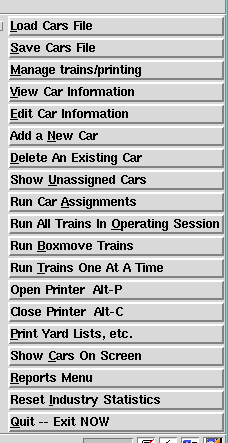
\includegraphics{FCFMainButtonMenu.png}
\caption{The Button Menu of the Freight Car Forwarder (V2) Program}
\label{fig:fcf:FCFMainButtonMenu}
\end{centering}
\end{figure}
\begin{figure}[hbpt]
\begin{centering}
\includegraphics{FCFMainIndicators.png}
\caption{The Indicators of the Freight Car Forwarder (V2) Program}
\label{fig:fcf:FCFMainIndicators}
\end{centering}
\end{figure}
The main GUI window\index{Freight Car Forwarder!main GUI}, show in
Figure~\ref{fig:fcf:FCFMain}, contains a menu bar, a toolbar
(Figure~\ref{fig:fcf:FCFMainToolbar}), a text display area, and a
button menu (Figure~\ref{fig:fcf:FCFMainButtonMenu}). There is also a 
work in progress message area, a  general status area, a progress
meter, and several indicators (Figure~\ref{fig:fcf:FCFMainIndicators}).
The main GUI also has three ``slide out'' frames, one for showing train
status when trains are run, one for viewing a car's information, and
one for editing a car's information. Each slide out has a corresponding
indicator. 

\section{Opening and loading a system file.}
\label{sect:fcf:loadsystem}
\index{Freight Car Forwarder!Loading a system file|(}

The \verb=File->Open...= menu button and the
\includegraphics{FCFLoadTool.png} toolbar button pop-up a file selection
dialog to select a system file to load. Once this file is successfully
loaded, the name of the file, the name of the system, the current
session and shift number, plus a count of  divisions, stations,
industries, cars, and trains is displayed in the main GUI's text area. 
Also all of the buttons are made active.  The name of the system file
can be specified on the command line and the named system file will be
loaded when the program starts.
\index{Freight Car Forwarder!Loading a system file|)}

\section{Loading and reloading the cars file.}

The \verb=Load Cars File= menu button and the

\includegraphics{FCFLoadCarsTool.png} toolbar button load (or reload)
the cars file.

\section{Saving the cars file.}

The \verb=Save Cars File= menu button and the 
\includegraphics{FCFSaveCarsTool.png} 
toolbar button save the cars and statistics files. This is something you
need to do after you have simulated a session, by running the car
assignment procedure and then run the trains in your session.  This
saves the state for the next time you run the Freight Car Forwarder.

\section{Managing trains and printing}
\begin{figure}[hbpt]
\begin{centering}
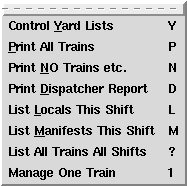
\includegraphics{FCFManageTrainsMenu.png}
\caption{Train/Printing Management Menu.}
\label{fig:fcf:FCFManageTrainsMenu}
\end{centering}
\end{figure}
The \verb=Manage trains/printing= menu button and the 
\includegraphics{FCFManageTrainsTool.png} toolbar button pop-up the
train/printing management menu.  This menu provides a set of functions
relating to what trains are printed and can also  print a dispatcher
report and generate lists of various sorts of trains.  The menu is shown
in  Figure~\ref{fig:fcf:FCFManageTrainsMenu}.

\subsection{Controling Yard Lists}

\begin{figure}[hbpt]
\begin{centering}
\includegraphics{FCFControlYardLDialog.png}
\caption{Control Yard Lists Dialog}
\label{fig:fcf:controlyardldialog}
\end{centering}
\end{figure}
The \verb=Control Yard Lists= menu item (y key) pops up a dialog, shown
in Figure~\ref{fig:fcf:controlyardldialog}, to control whether to print
0, 1, or 2 alphabetical lists and whether to print 0, 1, or 2 train
lists.

\subsection{Enabling printing for all trains}

The \verb=Print All Trains= menu item (p key) turns on printing for all
trains. 

\subsection{Disabling printing for all trains}

The \verb=Print No Trains= menu item (n key) turns off printing for all
trains.

\subsection{Printing a dispatcher report}

The \verb=Print Dispatcher Report= menu item (d key) enables the
printing of a dispatcher report.

\subsection{Listing local trains for this shift}

The \verb=List Locals This Shift= menu item (l key) lists all locals for
this shift.

\subsection{Listing manifests for this shift}

The \verb=List Manifests This Shift= menu item (m key) lists manifest
freights for this shift.

\subsection{Listing all trains for all shifts}

The \verb=List All Trains All Shifts= (? key) Lists all trains.

\subsection{Managing one train}

\begin{figure}[hbpt]
\begin{centering}
\includegraphics{FCFManage1TrainDialog.png}
\caption{Train Management Dialog}
\label{fig:fcf:manage1train}
\end{centering}
\end{figure}
The \verb=Manage One Train= menu item (1 key) pops up a dialog, shown
in Figure~\ref{fig:fcf:manage1train}, to enable or disable printing of
a single train, as well as setting the train's maximum length and
setting which shift the train will be run.  The train is selected with
the ``Select Train Dialog'', described in
Section~\ref{sect:fcf:selecttraindialog}.

\section{Viewing a car's information}

\begin{figure}[hbpt]
\begin{centering}
\includegraphics{FCFViewCarSlideout.png}
\caption{View Car Information Slideout}
\label{fig:fcf:viewcarslideout}
\end{centering}
\end{figure}
The \verb=View Car Information= menu button and the
\includegraphics{FCFViewCarTool.png} toolbar button display the
information about a single car.  The information is displayed on the
view car ``slide out'', shown in Figure~\ref{fig:fcf:viewcarslideout}.
The car is selected with the ``Search For Cars Dialog'', described in
Section~\ref{sect:fcf:searchcarsdialog}. 

\section{Editing a car's information}

\begin{figure}[hbpt]
\begin{centering}
\includegraphics{FCFEditCarSlideout.png}
\caption{Edit Car Information Slideout}
\label{fig:fcf:editcarslideout}
\end{centering}
\end{figure}
The \verb=Edit Car Information= menu button and the
\includegraphics{FCFEditCarTool.png} toolbar button display the
information about a single car and allow for editing this information. 
The information is displayed on the edit car ``slide out'', shown in
Figure~\ref{fig:fcf:editcarslideout}. The car is selected with the
``Search For Cars Dialog'', described in
Section~\ref{sect:fcf:searchcarsdialog}. 

\section{Adding a new car}

The \verb=Add a New Car= menu button and the
\includegraphics{FCFAddCarTool.png} toolbar button provide for adding a
new car.  The edit car ``slide out'', shown in
Figure~\ref{fig:fcf:editcarslideout} is displayed and the information
about the new car can be filled in and the car added.

\section{Deleting an existing car}

The \verb=Delete An Existing Car= menu button and the
\includegraphics{FCFDeleteCarTool.png} toolbar button provide for
deleting an existing car.  The car is selected with the ``Search For Cars
Dialog'', described in Section~\ref{sect:fcf:searchcarsdialog} and the
car's information is displayed in the view car ``slide out'', shown in
Figure~\ref{fig:fcf:viewcarslideout}. Actual removal can then be
confirmed.

\section{Showing cars without assignments}

The \verb=Show Unassigned Cars= menu button and the
\includegraphics{FCFShowUACarsTool.png} toolbar button display
unassigned cars in the text window.

\section{Running the car assignment procedure}

The \verb=Run Car Assignments= menu button and the
\includegraphics{FCFRunCarATool.png} toolbar button run the car
assignment procedure.  This procedure attempts to give as many
unassigned cars assignments, that is possible destinations. 
Considerations taken into account are the type of car, whether it is
loaded or not, industries with available trackage to accommodate the car,
and so on.  The list of cars is scanned twice and the progress of the
procedure is displayed in the text area.

\section{Running every train in the operating session}

\begin{figure}[hbpt]
\begin{centering}
\includegraphics{FCFTrainStatusSlideout.png}
\caption{Train Status Slideout}
\label{fig:fcf:trainstatusslideout}
\end{centering}
\end{figure}
The \verb=Run All Trains in Operating Session= menu button and the
\includegraphics{FCFRunAllTrTool.png} toolbar button run all trains in
the operating session, except the end of session box moves.  Each
train's progress is shown in the ``Train Status Slideout'', shown in
Figure~\ref{fig:fcf:trainstatusslideout}.

\section{Running the boxmove trains}

The \verb=Run Boxmove Trains= menu button and the
\includegraphics{FCFRunBTrTool.png} toolbar button run all of the box
move trains in the operating session.  Each train's progress is shown
in the ``Train Status Slideout'', shown in
Figure~\ref{fig:fcf:trainstatusslideout}.

\section{Running a single train}

The \verb=Run Trains One At A Time= menu button and the
\includegraphics{FCFRun1TrTool.png} toolbar button run a single train,
selected with the ``Select Train Dialog'', described in
Section~\ref{sect:fcf:selecttraindialog}. The train's progress is shown
in the ``Train Status Slideout'', shown in
Figure~\ref{fig:fcf:trainstatusslideout}.


\section{Opening a Printer}

\begin{figure}[hbpt]
\begin{centering}
\includegraphics{FCFOpenPrinterDialog.png}
\caption{Open Printer Dialog}
\label{fig:fcf:openprinterdialog}
\end{centering}
\end{figure}
The \verb=Open Printer= menu button and the
\includegraphics{FCFOpenPrinterTool.png} toolbar button open the printer
output file, using the ``Open Printer Dialog'', shown in
Figure~\ref{fig:fcf:openprinterdialog}. The status of the printer
output, open or closed, is shown with the printer status indication,
\includegraphics{FCFPrinterInd.png}.

\section{Closing the printer}

The \verb=Close Printer= menu button and the
\includegraphics{FCFClosePrinterTool.png} toolbar button close the
printer.The status of the printer output, open or closed, is shown with
the printer status indication, \includegraphics{FCFPrinterInd.png}.

\section{Printing yard and switch lists}

The \verb=Print Yard Lists, etc.= menu button and the
\includegraphics{FCFPrintYardTool.png} toolbar button print the yard and
switch lists.

\section{Showing cars on the screen}

\begin{figure}[hbpt]
\begin{centering}
\includegraphics{FCFShowCarsMenu.png}
\caption{Show Cars Menu}
\label{fig:fcf:showcarsmenu}
\end{centering}
\end{figure}
The \verb=Show Cars On Screen= menu button and the
\includegraphics{FCFShowCarsTool.png} toolbar button pops up a menu,
shown in Figure~\ref{fig:fcf:showcarsmenu}, of classes of cars to show.

\section{Printing Reports}

\begin{figure}[hbpt]
\begin{centering}
\includegraphics{FCFReportsMenu.png}
\caption{Reports Menu}
\label{fig:fcf:reportsmenu}
\end{centering}
\end{figure}
The \verb=Reports Menu= menu button and the
\includegraphics{FCFReportsTool.png} toolbar button pops up a menu,
shown in Figure~\ref{fig:fcf:reportsmenu}, of
possible reports.

\section{Reseting Industry Statistics}

The \verb=Reset Industry Statistics= menu button and the
\includegraphics{FCFResetStatsTool.png} toolbar button resets the
industry statistics.

\section{Quiting the application}

The \verb=Quit -- Exit NOW= menu button and the
\includegraphics{FCFCloseTool.png} toolbar button exit the program. A
confirmation dialog is popped up.


\section{General Dialogs}

\subsection{Control Yard Lists Dialog}
\subsection{Enter Owner Initials Dialog}

\subsection{Select A Train Dialog}
\label{sect:fcf:selecttraindialog}

\begin{figure}[hbpt]
\begin{centering}
\includegraphics{FCFSelectATrainDialog.png}
\caption{Select A Train Dialog}
\label{fig:fcf:selecttraindialog}
\end{centering}
\end{figure}
The Select a Train Dialog is used to select a train (to manage, run, or
print). The \verb=Filter= button uses the Train Name Pattern to match
against train names to select a subset of trains to select from and can
contain these special sequences:  
\begin{itemize} 
\item \verb=*= Matches any sequence of zero or more characters in the
train name.
\item \verb=?= Matches any single character in the train name. 
\item \verb=[chars]= Matches any character in the set given by chars. 
If a sequence of the form \verb=x-y= appears in chars, then any
character between \verb=x= and  \verb=y=,  inclusive,  will match.
Characters are matched in a case insensitive way. 
\item \verb=\x= matches the single character \verb=x=. This provides a 
way of avoiding the special interpretation of the characters
\verb=*?[]\= in the pattern.
\end{itemize}

\subsection{Manage One Train Dialog}
\subsection{Open Printer Dialog}

\subsection{Search For Cars Dialog}
\label{sect:fcf:searchcarsdialog}

\begin{figure}[hbpt]
\begin{centering}
\includegraphics{FCFSelectACarDialog.png}
\caption{Search For Cars Dialog}
\label{fig:fcf:searchcarsdialog}
\end{centering}
\end{figure}
The Search For Cars Dialog is used to select a car (to view, edit, or
delete). The \verb=Filter= button selects a  subset of cars based on the
trailing car number digits.

\subsection{Select A Division Dialog}
\subsection{Select An Industry Dialog}
\subsection{Select A Station Dialog}
\subsection{Select Car Type}

\section{Data files}
\label{sect:fcf:Files}

The Freight Car Forwarder uses a collection of eight data files:

\begin{enumerate}
\item \verb=System File= This is the \textbf{master} file.  It contains the
(relative) paths to the remaining seven files, along with the name of
the railroad system, its divisions, and its stations.

\item \verb=Industry File= This file holds the description of the
industries, both on-line, which are actually modeled on the layout and
off- line, which are imaginary industries not actually on the layout,
but might be modeled as implied by staging yards or by interchange with
other layouts or imaginary off-line railroads.

\item \verb=Trains File= This file holds the description of the trains used
to actually move the cars about the layout.

\item \verb=Orders File= This file contains standing train orders and is
only used to add additional information to the printouts given to trail
operators.

\item \verb=Owners File= This file contains a mapping between owner initials
and owner names.  Used with various generated reports.

\item \verb=Car Types File= This file contains a mapping between car type
codes and full names and descriptions of car types.

\item \verb=Cars File= This is the file containing information about all of
the rolling stock on or off the layout.

\item \verb=Statistics File= This is the statistics file.  It is generated
by the program and contains statistical information about car and
industry utilization.
\end{enumerate}


\subsection{Data File Formats}
\label{sect:fcf:File Formats}

Some general notes:

A comment it indicated by an apostrophe.  All characters from the
apostrophe to the end of the line are discarded when read.  The files
generally contain lines of comma separated fields, a format
designed for BASIC read statements--the original program that this
program is based on was written in a version of BASIC and uses the same
file format.

\subsubsection{System File}

The first line of the system file is the name of the railroad system. 
This line is used in various banners and report headings.

The second line should be a blank line.

Then come the names of the remaining seven data files, one per line, in
this order: \verb=Industry File=, \verb=Trains File=, \verb=Orders File=, 
\verb=Owners File=, \verb=Car Types File=, \verb=Cars File=, and finally 
\verb=Statistics File=. 

After the file names comes the division list.  This starts with a count
of the maximum number of divisions:

\begin{verbatim}
Divisions = Number
\end{verbatim}

where Number is a positive non zero integer.

This is followed by division specifications, which is a list of 5 values
separated by commas:

\begin{verbatim}
Number,Symbol,Home,Area,Name
\end{verbatim}

Where Number is the index of the division (between 1 and the max number
of divisions, inclusive), Symbol is an alphanumeric character (a-z, 0-9,
A-Z), Home is the number of the home yard for this division (must be a
yard specified in the \verb=Industry File=), area is an Area symbol, and
Name is the name of the division.

A line containing a -1 terminates the list of divisions.

Then comes the stations (cities), starting with a line defining the maximum
number of stations:

\begin{verbatim}
Stations = Number
\end{verbatim}

where Number is a positive non zero integer.

This is followed by station specifications, which is a list of 4 values
separated by commas:

\begin{verbatim}
Number,Name,Division,Comment
\end{verbatim}

Where Number is the index of the station (between 1 and the max number
of stations, inclusive), Name is the name of the city, Division is the
division index, and Comment is commentary about the station. 
City/Station number one is used for the workbench.

A line containing a -1 terminates the list of stations.

\subsubsection{Industry File}

The industry file contains industries and yards.  The file starts with a
line specifying the maximum number of industries:

\begin{verbatim}
Industries = Number
\end{verbatim}

where Number is a positive non zero integer.

Followed by a line for each industry or yard.  Industry number 0 is
used for the repair yard, which is for cars not in service.  Each
industry's line contains these fields:

\begin{verbatim}
ID,T,STA,NAME,TLEN,ALEN,P,R,H,MIR,C,W,DCL,MAX,LD,EM
\end{verbatim}

Where:

\begin{description}
\item[ID]    Numeric identifier.
\item[T]     Types are \textbf{Y}ard or \textbf{I}ndustry or \textbf{O}ffline.
\item[STA]   Station Identifier.
\item[NAME]  User friendly place name.
\item[TLEN]  Actual or virtual track length.
\item[ALEN]  Assignable length.
\item[P]     Priority for car assignments. If \textbf{YARD} or \textbf{STAGE}, 
	\textbf{P} is $n$, the number of yard lists to print of type \verb=A=, 
	\verb=P=, or \verb=D=.
\item[R]     Reloads cars \textbf{Y}es or \textbf{N}o.
\item[H]     Hazard class for outbound cargo.
\item[MIR]   Mirror industry or 0 if none.
\item[C]     Maximum clearance plate.
\item[W]     Maximum weight class.
\item[DCL]   Destination Control List of divisions. If \textbf{YARD} or 
\textbf{STAGE}, DCL can contain:
  \begin{description}
  \item[A]     Alphabetical listing of cars in yard is permitted.
  \item[P]     Pickup listing of cars in yard is permitted.
  \item[D]     Dropoff listing of cars in yard is permitted.
  \end{description}
\item[MAX]   Maximum allowed car length.
\item[LD]    Loaded car types accepted.
\item[EM]    Empty car types accepted.
\end{description}

The industry listing is terminated by a line containing a -1.

\subsubsection{Trains File}

The trains file contains the trains used to move the cars.  The file
starts with a line specifying the maximum number of trains:

\begin{verbatim}
Trains = Number
\end{verbatim}

where Number is a positive non zero integer.

Followed by a record for each train (a newline is acceptable alternative
to a comma):

{\footnotesize
\begin{verbatim}
Number,Type,Shift,Done,Name,Maxcars, Divisions, Stops
	filler,Onduty,Print,Maxclear, Maxweight, Types,  Maxlen, 
	Description
\end{verbatim}
}

Where Number is the train number, Type is \textbf{M}anifest;
\textbf{B}oxmove; \textbf{W}ayfreight; or \textbf{P}assenger, Shift is
1; 2; or 3, Done is \textbf{Y}es or \textbf{N}o, Name is the train
name, Maxcars is the maximum number of cars, Divisions is a set of
division symbols or a wildcard (\verb=*=),Stops is a space separated
list of stations (Boxmove and Wayfrieghts) or industries (Manifests),
filler is an unused slot (use 0), Onduty is the time on duty (the
train's departure time) in the format HHMM, Print is \textbf{P}rint or
\textbf{N}oprint, Maxclear is the maximum clearance number, Maxweight
is the maximum weight number, Types is a set of car types this train
can carry, Maxlen is the maximum train length in feet, and Description
is a textual description of the train.

The train listing is terminated by a line containing a -1.

\subsubsection{Orders File}

This file contains lines with pairs:

\begin{verbatim}
Name,Order
\end{verbatim}

where Name is the name of a train and Order is a quoted string
containing the order.

\subsubsection{Owners File}

This file starts with a count of owners and then lines with with
triples:

\begin{verbatim}
Initials,Name,Comment
\end{verbatim}

where Initials are the three letter initials of an owner, Name is the
full name of the owner, and Comment is some descriptive text.

\subsubsection{Car Types File}

This is a file with exactly 91 records.  Each record contains:

\begin{verbatim}
Car Type Code,Car Type Group,Description,pad,Comment
\end{verbatim}

where Car Type Code is one of 91 printable characters, Car Type Group
is a single character, Description is a 16 character brief description,
pad is 0, and Comment is some descriptive text.

After the car types is the Car type groupings, which map groups of car
types into groups using the second single character, with lines
containing these fields:

\begin{verbatim}
Car Type Group,Description,Comment
\end{verbatim}

where Car Type Group is a single character, Description is a 16
character brief description, and Comment is some descriptive text.

\subsubsection{Cars File}

The cars file starts with three numbers, one per line:

\begin{verbatim}
Total shifts
Current shift
Max car count
\end{verbatim}

The first number is the total number of shifts, the second is the
current shift number (1, 2, or 3), and the third number is the maximum
number of cars in the file.

The remainder of the file is car records. This file must be kept in
[alphabetical order]! Each record contains:

{\footnotesize
\begin{verbatim}
Type,Marks,Number,Home,CarLen,ClearPlate,CarWeight,EmptyWt,
	LoadLimit,Loaded,Mirror?,Fixed?,Owner,Done,Last,Moves,Loc,
	Dest,NTrips,NAssigns
\end{verbatim}
}
Where Type is from car types file, Marks is the railroad reporting
marks (9 characters max), Number is the car number (8 characters max),
Home is car home division (from system file), CarLen is extreme car
length, ClearPlate is the clearance plate (from plate file), CarWeight
is car weight class (from weight file), EmptyWt is light weight in
tons, LoadLimit is load limit in tons, Loaded is \textbf{L}loaded or
\textbf{E}mpty, Mirror? is ok to mirror \textbf{Y}es or \textbf{N}o,
Fixed? is fixed route \textbf{Y}es or \textbf{N}o, Owner is car owner's
3 character initials (from owners file), Done is car is done moving for
this session \textbf{Y}es or \textbf{N}o, Last is last train to handle
the car from trains file,Moves is actual movements this session,Loc is
car's present location from industry file, Dest car's destination from
industry file, NTrips is number of car trips, and NAssigns is number of
car assignments.

\subsubsection{Statistics File}

The statistics is a file generated as an output and should not be hand
edited.  This file has two formats, V1 and V2.  V1 is the original
format used by the original BASIC program.  V2 is an improved version
that avoids getting the fields jammed together due to numerical overflow
(result numbers too large for the field sizes).

The first line of either format contains the statistics period number. 
If in the new format (V2), this number is followed by a comma.

The rest of file file contains lines of four numbers, either space
separated (V1) or comma separated (V2): industry index, car count, car
length, and statistics length.

\subsubsection{Other data files}

There are some additional data files, which are not actually loaded into
the system.  These are the plate, weight, and hazard files.  These are
just informational files that are used to map clearance plate, weight
class, and hazard levels of cars.




\part{Calculation Scripts}
\label{part:calc}
%* 
%* ------------------------------------------------------------------
%* ResistorManual.tex - Resistor Manual
%* Created by Robert Heller on Wed Mar 19 14:53:24 2008
%* ------------------------------------------------------------------
%* Modification History: $Log$
%* Modification History: Revision 1.1  2002/07/28 14:03:50  heller
%* Modification History: Add it copyright notice headers
%* Modification History:
%* ------------------------------------------------------------------
%* Contents:
%* ------------------------------------------------------------------
%*  
%*     Model RR System, Version 2
%*     Copyright (C) 1994,1995,2002-2005  Robert Heller D/B/A Deepwoods Software
%* 			51 Locke Hill Road
%* 			Wendell, MA 01379-9728
%* 
%*     This program is free software; you can redistribute it and/or modify
%*     it under the terms of the GNU General Public License as published by
%*     the Free Software Foundation; either version 2 of the License, or
%*     (at your option) any later version.
%* 
%*     This program is distributed in the hope that it will be useful,
%*     but WITHOUT ANY WARRANTY; without even the implied warranty of
%*     MERCHANTABILITY or FITNESS FOR A PARTICULAR PURPOSE.  See the
%*     GNU General Public License for more details.
%* 
%*     You should have received a copy of the GNU General Public License
%*     along with this program; if not, write to the Free Software
%*     Foundation, Inc., 675 Mass Ave, Cambridge, MA 02139, USA.
%* 
%*  
%* 

\chapter{Resistor Program Reference}
\label{chpt:rest:Reference}
\typeout{$Id$}

The Resistor Calculator program aids in calculating dropping resistors
for LEDs and low-voltage lamps commonly used on model railroads.  It
implements Ohm's Law\index{Ohm's Law}, shown in
Equations~\ref{eq:rest:OhmsLaw} and~\ref{eq:rest:VDrop} to perform the
calculation and then finds the nearest stock value and also displays
the color bands for typical carbon resistors.

\begin{eqnarray}
R_{drop} &=& \frac{V_{drop}}{I} \label{eq:rest:OhmsLaw} \\
V_{drop} &=& V_{supply} - V_{load} \label{eq:rest:VDrop}
\end{eqnarray}

The calculator takes three input values, the supply voltage
($V_{supply}$), the voltage across the load ($V_{load}$) (LED or lamp)
and the load current ($I$) the LED or lamp operates at.  These values
are entered along with the units they are in. Then the calculate button
is pushed and the results are displayed.  The results can also be saved
to a text file, which can be printed or otherwise refered to later.

\begin{figure}[hbpt]
\begin{centering}
\includegraphics[width=5in]{RestMain.png}
\caption{The main GUI screen of the Resistor Calculator program}
\label{fig:rest:Main}
\end{centering}
\end{figure}
The main GUI screen of the Resistor Calculator program is shown in
Figure~\ref{fig:rest:Main}.  


%* 
%* ------------------------------------------------------------------
%* LocoPullManual.tex - LocoPull Manual
%* Created by Robert Heller on Mon Mar 22 15:23:08 2010
%* ------------------------------------------------------------------
%* Modification History: $Log$
%* Modification History: Revision 1.1  2002/07/28 14:03:50  heller
%* Modification History: Add it copyright notice headers
%* Modification History:
%* ------------------------------------------------------------------
%* Contents:
%* ------------------------------------------------------------------
%*  
%*     Model RR System, Version 2
%*     Copyright (C) 1994,1995,2002-2005  Robert Heller D/B/A Deepwoods Software
%* 			51 Locke Hill Road
%* 			Wendell, MA 01379-9728
%* 
%*     This program is free software; you can redistribute it and/or modify
%*     it under the terms of the GNU General Public License as published by
%*     the Free Software Foundation; either version 2 of the License, or
%*     (at your option) any later version.
%* 
%*     This program is distributed in the hope that it will be useful,
%*     but WITHOUT ANY WARRANTY; without even the implied warranty of
%*     MERCHANTABILITY or FITNESS FOR A PARTICULAR PURPOSE.  See the
%*     GNU General Public License for more details.
%* 
%*     You should have received a copy of the GNU General Public License
%*     along with this program; if not, write to the Free Software
%*     Foundation, Inc., 675 Mass Ave, Cambridge, MA 02139, USA.
%* 
%*  
%* 

\chapter{LocoPull Program Reference}
\label{chpt:locopull:Reference}
\typeout{$Id$}

\section{Basis and Mathematics}
This program is based on the information posted by Mark U. on the Yahoo
XTrkCad list\footnote{At the URL
\url{http://groups.yahoo.com/group/XTrkCad/message/4983}.} and the
information supplied by rtroop on the TrainBoard forum\footnote{Post
\#9 at the URL
\url{http://www.trainboard.com/grapevine/showthread.php?t=114497}.}.
This is a standalone program that incorporates the formulas presented in
Mark U's spreadsheet and explained in rtroop's message.  The formulas
are as follows:

\begin{eqnarray}
E_{unit} &=& W_{unit}{A} \label{eq:locopull:teperunit} \\
E  &=& E_{unit}{N} \label{eq:locopull:tenet} \\
R_{ave}  &=& W_{ave}{F} \label{eq:locopull:aveRR} \\
C_{0~Grade} &=& \Biggl\lfloor \frac{E}{R_{ave}} \Biggr\rfloor \label{eq:locopull:zgrade} \\
R_{grade}    &=& W_{ave}{G} \label{eq:locopull:rraddedgrade} \\
R_{net~at~grade} &=& R_{ave} + R_{grade} \label{eq:locopull:rratgrade} \\
R_{unit~at~grade} &=& W_{unit}{G} \label{eq:locopull:rrunitgrade} \\
D &=& \frac{5730}{\frac{rS}{12}} \label{eq:locopull:degreecurve} \\
C_{grade~and~curve} &=& \Biggl\lfloor 
     \frac{ {E} - {N} {W_{unit}} ( G + F + D ) }
          { {R_{ave}} + {W_{ave}} ( G + {F_{per~degree}}
							{D} ) } 
	\Biggr\rfloor \label{eq:locopull:capatgradecurve}
\end{eqnarray}



\begin{tabular}{rrp{3in}}
Where:&&\\
&$W_{unit}$ &is the weight of each locomotive in ounces. \\
&$A$ &is the adhesion factor generally 25\%. \\
&$E_{unit}$&is the tractive effort per unit in ounces. \\
&$E$&is the net tractive effort in ounces. \\
&$N$&is the number of units. \\
&$F$ &is the resistance factor of each car, typically 4\% for N
scale cars.\\
&$W_{ave}$&is the average weight per car, typically 1 ounce for N scale cars.\\
&$R_{ave}$&is the average rolling resistance of each car.\\
&$C_{0~Grade}$&is the capacity of the train on level, straight
track.\\
&$G$&is the percent of grade.\\
&$R_{grade}$&is the added rolling resistance of each car due to
grade.\\
&$R_{net~at~grade}$&is the net rolling resistance of each car at
grade.\\
&$r$ &is the track radius in inches.\\
&$S$&is the scale factor (160 for N scale, 87 for H0 scale, etc.).\\
&$D$& is the degree of curvature.\\
&$F_{per~degree}$&is the resistance factor per degree of curvature,
typically .04\%.\\
&$C_{grade~and~curve}$&is the capacity of the train on at grade on a
curve.\\
\end{tabular}

\section{The GUI}
\begin{figure}[hbpt]
\begin{centering}
\includegraphics[width=5in]{LocoPullMain.png}
\caption{The main GUI screen of the LocoPull program}
\label{fig:locopull:main}
\end{centering}
\end{figure}
The main GUI screen of the LocoPull program is shown in
Figure~\ref{fig:locopull:main}. The GUI is broken down into sections: 
\begin{itemize}
\item The Scale section.  The scale is selected here.
\item The Locomotive Information section.  Information about the
locomotives is entered here.  The number of locomotives, how much they
weigh each, and their adhesion factor. The tractive effort for each unit
and the net tractive effort are computed and displayed here. It is
assumed that all of the powered engines are the same, typically the same
make and model, with the same weight and same adhesion factor.
\item The Consist Information. Information about the cars, including
their average weight and their average resistance factor are entered and
the rolling rolling resistance is computed and displayed.
\item The Zero-grade Capacity section.  The maximum number of cars that
can be pulled on a straight track on a level grade is computed and
displayed here.
\item The Grade Information section. The percent of grade is entered and
the added rolling resistance per car at grade, the net rolling
resistance, and the added resistance per unit are computed and displayed
here. 
\item The Curve Information section. The radius of the curve in inches
and the rolling resistance per degree of curve are entered and the
degree of curvature is computed and displayed.
\item The Capacity at Grade and Curve section.  This is the maximum
number of cars that can be pulled at the grade and curve specified.
\item Calculate button. This button performs the calculation and updates
all of the displayed values.
\end{itemize}

\subsection{The Scale}
The scale selection simply select the scale and is used to compute the
degree of curvature.

\subsection{Locomotive Information}
This section of the GUI gathers information about the locomotives
pulling the train.  It is assumed that all of the locomotives have the
same tractive effort, that is they are the same weight and have the same
adhesion factor.  This would generally be the case if the locomotives
were the make and model.  Three inputs are gathered in this section: the
number of locomotives, the weight of each locomotive, and the adhesion
factor of the locomotives.  Two intermediate outputs are displayed here:
the tractive effort of each locomotive and the net tractive effort of
all of the locomotives together.

\subsection{Consist Information}
This section gathers two inputs and displays one intermediate result. 
The two inputs are the average weight of the cars and the average
rolling resistance factor.  The intermediate result is the average car
rolling resistance.

\subsection{Zero-grade capacity}
This is simply the net tractive effort divided by the average car
rolling resistance.  The floor of the result is displayed as a whole
number (since pulling a fraction of a car is not meaningful).

\subsection{Grade information}
One input is gathered and three intermediate results are displayed.  The
input is the percent of grade and the intermediate results displayed are
the added rolling resistance at grade of each car, the net rolling
resistance per car, and the added rolling resistance of each locomotive
at grade.

\subsection{Curve information}
This section gathers two inputs and displays one intermediate result.
The added inputs are the curve radius and the rolling resistance per
degree of curvature and the intermediate result is the degree of
curvature. 

\subsection{Capacity and Grade plus Curve}
This is just the tractive effort less the tractive effort needed to
pull the locomotives themselves divided by the combined rolling
resistance of the average car: base rolling resistance plus the added
rolling resistance due to grade, plus the added rolling resistance due
to the curvature.  The floor of the result is displayed as a whole
number (since pulling a fraction of a car is not meaningful).





\part{Camera Scripts}
\label{part:camera}
\include{AnyDistanceManual}
\include{ClosestManual}

%* 
%* ------------------------------------------------------------------
%* DispatcherPart.tex - Dispatcher User Manual
%* Created by Robert Heller on Wed May 28 17:08:00 2008
%* ------------------------------------------------------------------
%* Modification History: $Log$
%* Modification History: Revision 1.1  2002/07/28 14:03:50  heller
%* Modification History: Add it copyright notice headers
%* Modification History:
%* ------------------------------------------------------------------
%* Contents:
%* ------------------------------------------------------------------
%*  
%*     Model RR System, Version 2
%*     Copyright (C) 1994,1995,2002-2005  Robert Heller D/B/A Deepwoods Software
%* 			51 Locke Hill Road
%* 			Wendell, MA 01379-9728
%* 
%*     This program is free software; you can redistribute it and/or modify
%*     it under the terms of the GNU General Public License as published by
%*     the Free Software Foundation; either version 2 of the License, or
%*     (at your option) any later version.
%* 
%*     This program is distributed in the hope that it will be useful,
%*     but WITHOUT ANY WARRANTY; without even the implied warranty of
%*     MERCHANTABILITY or FITNESS FOR A PARTICULAR PURPOSE.  See the
%*     GNU General Public License for more details.
%* 
%*     You should have received a copy of the GNU General Public License
%*     along with this program; if not, write to the Free Software
%*     Foundation, Inc., 675 Mass Ave, Cambridge, MA 02139, USA.
%* 
%*  
%* 

\typeout{$Id$}

\part{Dispatcher}
\label{part:dispatch}
%* 
%* ------------------------------------------------------------------
%* DispatcherTutorial.tex - Dispatcher Tutorial
%* Created by Robert Heller on Wed May 28 17:16:26 2008
%* ------------------------------------------------------------------
%* Modification History: $Log$
%* Modification History: Revision 1.1  2002/07/28 14:03:50  heller
%* Modification History: Add it copyright notice headers
%* Modification History:
%* ------------------------------------------------------------------
%* Contents:
%* ------------------------------------------------------------------
%*  
%*     Model RR System, Version 2
%*     Copyright (C) 1994,1995,2002-2005  Robert Heller D/B/A Deepwoods Software
%* 			51 Locke Hill Road
%* 			Wendell, MA 01379-9728
%* 
%*     This program is free software; you can redistribute it and/or modify
%*     it under the terms of the GNU General Public License as published by
%*     the Free Software Foundation; either version 2 of the License, or
%*     (at your option) any later version.
%* 
%*     This program is distributed in the hope that it will be useful,
%*     but WITHOUT ANY WARRANTY; without even the implied warranty of
%*     MERCHANTABILITY or FITNESS FOR A PARTICULAR PURPOSE.  See the
%*     GNU General Public License for more details.
%* 
%*     You should have received a copy of the GNU General Public License
%*     along with this program; if not, write to the Free Software
%*     Foundation, Inc., 675 Mass Ave, Cambridge, MA 02139, USA.
%* 
%*  
%* 

\chapter{Dispatcher Tutorial}
\label{chpt:dispatcher:Tutorial}
\typeout{$Id$}

\section{A ``Simple Mode'' CTC Panel}


\begin{figure}[hbpt]
\begin{centering}
\includegraphics{DISPSimpleTutNewCTC.png}
\caption{Creating a new Simple Mode CTC Panel}
\label{fig:dispatcher:Tut:newSimplePanel}
\end{centering}
\end{figure}
\begin{figure}[hbpt]
\begin{centering}
\includegraphics[width=5in]{DISPSimpleTutBlankCTC.png}
\caption{Initial blank panel}
\label{fig:dispatcher:Tut:blankPanel}
\end{centering}
\end{figure}
%
This tutorial will go through the steps of creating a simple CTC panel
for a passing siding.  First, after starting up the Dispatcher program,
we will click on the \texttt{New CTC Window} toolbar button and get a
\texttt{New CTCPanel} dialog box, as shown in
Figure~\ref{fig:dispatcher:Tut:newSimplePanel}. See
Section~\ref{sect:dispatcher:creatingCTCPanels} for more information.
We fill in a name and select the \texttt{Simple Mode} check button.
Clicking on \texttt{Create} gives us the blank panel shown in
Figure~\ref{fig:dispatcher:Tut:blankPanel}. Now we can start adding
track work and control elements.  But first a brief discussion about how
things are structured.  First of all every object has a unique name and
every object is in a named control point.  A ``control point'' is a
collection of track work elements and control panel elements that relate
to a single controlled feature, typically a turnout of some sort. The
control point usually includes a code button, which is a button that
initiates some change in the track work (turnouts, signals, etc.), based
upon the settings of one or more control panel elements.  In this
tutorial we will be creating four control points, \textbf{CP1},
\textbf{CP2}, \textbf{Main}, and \textbf{Siding}.  \textbf{CP1} is the
turnout at the Western (left) end of the siding, \textbf{CP2} is the
turnout at the Eastern (right) end of the siding, \textbf{Main} is the
mainline trackage, and \textbf{Siding} is the siding track. The
\textbf{Main} and \textbf{Siding} control points won't have any control
panel objects and are only being used to contain the simple track
elements. These are essentially ``dummy'' control points and are just
being used as containers for track work that does not contain any
centrally controllable track work.

\begin{figure}[hbpt] 
\begin{centering}
\includegraphics[width=4in]{DISPSimpleTutSw1.png} 
\caption{Creating Turnout 1}
\label{fig:dispatcher:Tut:Sw1} 
\end{centering} 
\end{figure}
%
\begin{figure}[hbpt] 
\begin{centering}
\includegraphics[width=4in]{DISPSimpleTutSw1CrossHairs.png} 
\caption{Positioning Turnout 1} 
\label{fig:dispatcher:Tut:Sw1CrossHairs} 
\end{centering}
\end{figure} 
%
\begin{figure}[hbpt] 
\begin{centering}
\includegraphics[width=4in]{DISPSimpleTutPanel1.png} 
\caption{Turnout 1 placed on the panel} 
\label{fig:dispatcher:Tut:panel1} 
\end{centering}
\end{figure} 
%
First we will create turnout 1 (named \textbf{Switch1}) by selecting
\texttt{Add Object} on the \texttt{Panel} menu, which gives us the
\texttt{Add Panel Object to panel} dialog box, shown in
Figure~\ref{fig:dispatcher:Tut:Sw1}. See
Section~\ref{sect:dispatcher:addeditdeletePanelElements} for more
information. We will ``flip'' the turnout to give it the proper
orientation. Turnouts can be flipped and can also be rotated to one of
eight positions (45 degree increments). We will use the cross hairs to
roughly position the turnout, as shown in
Figure~\ref{fig:dispatcher:Tut:Sw1CrossHairs}. Clicking the
\texttt{Add} button places the turnout on the track work schematic, as
shown in  Figure~\ref{fig:dispatcher:Tut:panel1}.  \begin{tip}You can
fine tune the location of the object by making small changes to the X
and Y coordinates after you have roughly placed the object using the
cross hairs. You can always go back and edit an object by using the
\texttt{Edit Object} menu item on the \texttt{Panel} menu and then
selecting the name of the object to edit.\end{tip}

\clearpage

\begin{figure}[hbpt] 
\begin{centering}
\includegraphics[width=4in]{DISPSimpleTutSWPlate1.png} 
\caption{Adding a Switch Plate} 
\label{fig:dispatcher:Tut:SWPlate1}
\end{centering}
\end{figure} 
%
\begin{figure}[hbpt] 
\begin{centering}
\includegraphics[width=4in]{DISPSimpleTutPanel2.png} 
\caption{Switch Plate 1 placed on the panel} 
\label{fig:dispatcher:Tut:panel2} 
\end{centering}
\end{figure} 
%
Next, we will add a switch plate (named \textbf{SwitchPlate1}), again
by selecting \texttt{Add Object} on the \texttt{Panel} menu, again
using the \texttt{Add Panel Object to panel} dialog box, shown in
Figure~\ref{fig:dispatcher:Tut:SWPlate1}. We will enter the name of the
turnout it controls (\textbf{Switch1}) and the serial number of the
MRD2-U board that will be controlling the Switch-It board powering the
switch motor. Again we will use the cross hairs to place the switch
plate. The result is shown in Figure~\ref{fig:dispatcher:Tut:panel2}.

\clearpage

\begin{figure}[hbpt] 
\begin{centering}
\includegraphics[width=4in]{DISPSimpleTutCB1.png} 
\caption{Adding a code button} 
\label{fig:dispatcher:Tut:CB1}
\end{centering}
\end{figure} 
%
\begin{figure}[hbpt] 
\begin{centering}
\includegraphics[width=4in]{DISPSimpleTutPanel3.png} 
\caption{Code button 1 placed on the panel} 
\label{fig:dispatcher:Tut:panel3} 
\end{centering}
\end{figure} 
%
Finally, we will add a code button, as shown in
Figures~\ref{fig:dispatcher:Tut:CB1} and
~\ref{fig:dispatcher:Tut:panel3}.

\clearpage

\begin{figure}[hbpt] 
\begin{centering}
\includegraphics[width=5in]{DISPSimpleTutPanel4.png} 
\caption{The completed panel} 
\label{fig:dispatcher:Tut:Panel4} 
\end{centering}
\end{figure} 
%
We repeat this process to add the mainline, the siding, and the second
turnout, with its switch plate and code button. \begin{tip}Place the
second turnout next, then add the mainline and the siding tracks. Once
the turnouts have been placed, the locations of the endpoints of the
straight track sections are easy to select.\end{tip} Finally we get the
panel shown in Figure~\ref{fig:dispatcher:Tut:Panel4}.

Once the panel has been completed, we can use the \texttt{Wrap As} menu
item under the \texttt{File} menu to create a ``wrapped'' version of
the generated program.  This is a self-contained, stand-alone
executable program that implements the CTC panel. See
Section~\ref{sect:dispatcher:wrapas} for more information.



%%\section{A more advanced Example}

%* 
%* ------------------------------------------------------------------
%* DispatcherReference.tex - Dispatcher Reference
%* Created by Robert Heller on Wed May 28 18:01:28 2008
%* ------------------------------------------------------------------
%* Modification History: $Log$
%* Modification History: Revision 1.1  2002/07/28 14:03:50  heller
%* Modification History: Add it copyright notice headers
%* Modification History:
%* ------------------------------------------------------------------
%* Contents:
%* ------------------------------------------------------------------
%*  
%*     Model RR System, Version 2
%*     Copyright (C) 1994,1995,2002-2005  Robert Heller D/B/A Deepwoods Software
%* 			51 Locke Hill Road
%* 			Wendell, MA 01379-9728
%* 
%*     This program is free software; you can redistribute it and/or modify
%*     it under the terms of the GNU General Public License as published by
%*     the Free Software Foundation; either version 2 of the License, or
%*     (at your option) any later version.
%* 
%*     This program is distributed in the hope that it will be useful,
%*     but WITHOUT ANY WARRANTY; without even the implied warranty of
%*     MERCHANTABILITY or FITNESS FOR A PARTICULAR PURPOSE.  See the
%*     GNU General Public License for more details.
%* 
%*     You should have received a copy of the GNU General Public License
%*     along with this program; if not, write to the Free Software
%*     Foundation, Inc., 675 Mass Ave, Cambridge, MA 02139, USA.
%* 
%*  
%* 


\chapter{Dispatcher Reference}
\label{chpt:dispatcher:Reference}
\typeout{$Id$}

The Dispatcher program is used to create computerized CTC (Centralized
Traffic Control) panels, to be used by dispatchers as part of a CATC
(Computer Assisted Traffic Control) system to manage traffic flow for a
model railroad.  A computerized CTC panel typically contains a track work
schematic and a collection of control elements (such as switch plates,
signal plates, toggle switches, push buttons, etc.) that control the
track work and track side signals.  In addition to creating and editing
CTC panels, the Dispatcher program can read in an XTrkCAD layout file
and create a compressed graph of the track work and this graph can be
used as a guide while creating CTC panels.

\section{Main GUI Screen}

\begin{figure}[hbpt]
\begin{centering}
\includegraphics[width=5in]{DISPMainGUI.png}
\caption{Main Dispatcher Window}
\label{fig:dispatcher:mainDispatcher}
\end{centering}
\end{figure}
The main GUI window of the Dispatcher program is shown in
Figure~\ref{fig:dispatcher:mainDispatcher}. It consists of a standard
menu bar, a tool bar, and an area for track work graph display. A
track work graph is something computer scientists call a ``directed
graph''.  A directed graph is a data structure consisting of nodes,
with links to other nodes.  In this case each node is a piece of
track work and the links are the connections between pieces of track work
and thus indicate the adjacency of track work nodes (and how the pieces
of track work interconnect with each other).  In the case of simple
track work (such as straight sections or curved sections), there are one
(if the section ``dead ends'') or two links and in the case of complex
track work (such as turnouts and crossings), there are three or more
links.  The graph is ``compressed'', where adjacent pieces of simple
track work are consolidated into single nodes. 

\subsection{Track work Node Graphs}

Once the compressed graph is built (upon loading a layout file), it is
displayed on the main GUI screen as numbered circles (nodes) connected
by lines with arrows (links).  A graphic of the piece of track work is
also drawn. Left clicking on a node displays a pop-up containing
information about the track work node.  Right clicking on a node pops up
a menu of actions involving the node\footnote{Current two menu items
are defined, one to display the node info and the other to add it to a
panel.}. Left clicking on a link displays a pop-up containing
information about the link.  The node numbers are the track element
numbers assigned by XTrkCad.

\subsubsection{Loading a Layout}

An XTrkCAD layout file is loaded either with the \verb=Load XTrkCad File=
tool bar button or with the \verb=Load...= item on the \verb=File=
menu. It is also possible to load a XTrkCAD layout file during
program startup using the \verb=-xtrkcad= command line option.

In all cases, the layout's track work is loaded a track work graph and
displayed in the track work graph display area.  Dispatcher then asks if
XTrkCad itself should be started.  This might be useful as it gives a
display of the actual layout on your screen, which can be referred to
when creating CTC panels.

\subsubsection{Finding Nodes}

A node can be ``found'' by its number.  Finding a node scrolls the node
graph to make the node visible and the node is highlighted.

\subsubsection{Printing Node Graphs}

A node graph can be printed to provide a hard-copy reference of the node
graph.

\subsection{Creating a new CTC Panel}
\label{sect:dispatcher:creatingCTCPanels}

\begin{figure}[hbpt] \begin{centering}
\includegraphics{DISPNewCTCPanel.png} \caption{New CTC Panel Dialog}
\label{fig:dispatcher:newCTCPanel} \end{centering} \end{figure} A new
CTC Panel is created with the \verb=New CTC Window= too bar button or
the \verb=New CTC Panel Window= entry under the \verb=File= menu.  A
New CTC Panel Dialog, as shown in
Figure~\ref{fig:dispatcher:newCTCPanel}, is displayed. This dialog box
asks the user for some basic information about the new panel.  This
includes the name (title) of the panel, its initial width and height,
whether it connects to a C/MRI bus and information about that bus, as
well as whether it uses MRD devices\footnote{MRD2-U or MRD2-S devices,
made by Azatrax.}. 

There is also a checkbutton to select ``Simple Mode''.  ``Simple Mode''
simply means that the panel will be a simple one with canned code to
use Azatrax USB devices to actuate switch machines, either directly or
via NCE's Switch-It (or similar) units. The canned and auto-generated
code associates a Switch Plate with a switch and associates a Code
Button with 1 or more Switch Plates and Signal Plates\footnote{The
Signal Plates don't do anything but change their panel lights.}  In
``Simple Mode'', all of the UI elements relating to writing Tcl code
are disabled and all of the Tcl code is completely generated by the
Dispatcher program.  All the user does is place the trackwork elements
on the schematic and the control elements on the control panel and
provide some the serial number of the MRD2-U devices that are wired to
the Switch-Its and the names of the track work devices being controled.

What is actually created is a Tcl/Tk program that uses parts of the
library of Tcl/Tk and C++ code included with the Model Railroad System
that will implement a CTC Panel, which contains two display sections: a
track work schematic and a control panel.  The track work schematic is in
the upper half of the panel and has a black background with white (red
when occupied) track work. Signals with one, two, or three heads can be
added to the track work schematic.  The control panel is in the lower
half and has a dark green background. The control panel can have switch
plates, signal plates, toggle switches, push buttons, code buttons, and
indicator lamps.

The CTC Panel can be used by a dispatcher using a computer screen and
pointing device (such as a mouse or touch pad) to select and manipulate
control elements. The track work on a CTC Panel will reflect the actual
track conditions (occupied or not, signal aspects, and turnout states).

\subsection{Opening an existing CTC Panel}

Existing CTC Panel programs are the specifically formatted Tcl/Tk
programs created by the Dispatcher program.  They can be opened and
edited using the \verb=Open CTC File= too bar button or the
\verb=Open...= entry under the \verb=File= menu or specified on the
Dispatcher's command line.  There are three sections of the code that
are ``loaded'' into the Dispatcher program: the collection of CTC Panel
elements, the information about the (optional) C/MRI network or Azatrax
USB devices, and the user code associated with the panel.

\section{Configurable Options}
\label{sect:dispatcher:configopts}

The configurable options can be set or changed with the 
\verb=Edit Configuration= menu entry under the \verb=Options= menu. These
configurable options can be saved with the \verb=Save Configuration=
menu entry under the \verb=Options= menu and can be loaded with the 
\verb=Load Configuration= menu entry.  At present there are three
configuration options: \verb=Use External Editor=, which has a boolean
value (true or false), \verb=External Editor=, which is a
command line that starts an external editor (the name of the file
to edit is appended to this command line), and \verb=Tcl Kit=, which is
the name of the Tclkit file to use for the runtime when wraping panel
programs (see Section~\ref{sect:dispatcher:wrapas}).

\section{CTC Panel Windows}

\begin{figure}[hbpt]
\begin{centering}
\includegraphics[width=5in]{DISPEmptyCTCPanel.png}
\caption{Empty CTC Panel Window}
\label{fig:dispatcher:emptyCTCPanel}
\end{centering}
\end{figure}
A freshly created CTC Panel window is shown in
Figure~\ref{fig:dispatcher:emptyCTCPanel}\footnote{When the program is
run on its own, the Panel and C/Mri menus will be absent.}. The pink
square at the lower left indicates that the file is in a modified state
and has not been saved to disk.  Saving the file is done with the
\verb=Save= and \verb=Save As...= menu items under the \verb=File= menu.
It is also possible to create a standalone executable program file using
the \verb=Wrap As...= menu item under the \verb=File= menu (see
Section~\ref{sect:dispatcher:wrapas} for more information).

\subsection{Menu items available when editing a CTC Panel Window}

\subsubsection{File menu}

The \verb=File= contains entries to create a new CTC Panel Window, load
an XTrkCad file, open a CTC Panel Window, save the current CTC Panel
Window, wrap the current CTC Panel Window, close the current CTC Panel
Window, and exit.  Attempting to close a modified CTC Panel Window will
cause a save confirmation window, allowing you to save your work.

\subsubsection{Edit menu}

In addition to the standard edit menu entries, there are three extra
entries\footnote{These items are disabled when in ``Simple Mode''.}:

\begin{description}
  \item[(Re-)Generate Main Loop] This entry generates (or regenerates)
the main loop.  The basic loop read all of the input ports of all of the
C/MRI nodes, invokes all of the track work elements, and then writes all
of the output ports of all of the C/MRI nodes.  The loop is an endless
real time loop.  It is necessary to ``fill in'' the logic of the CTC Panel.
  \item[User Code] This entry opens an editor to edit the user code
section of the CTC Panel program.
  \item[Modules] This entry inserts selected helper modules into the
user code section of the CTC Panel program.  These are all in namespaces
and are SNIT types:
    \begin{description}
      \item[Track Work types] This inserts two SNIT types, one for
blocks (usable for simple track work) and one for switches (turnouts).
      \item[Switch Plate type] This inserts a SNIT type to handle switch
plates. 
      \item[Signals] This inserts SNIT types to help with signals:
	\begin{description}
	   \item[Two Aspect Color Light] Use this module if you are
using two lamp or LED (red and green) signals.  One, two, and three head
signals are supported.
	   \item[Three Aspect Color Light] Use this module if you are
using three  lamp or LED (red,  yellow,  and green) signals.  One, two,
and three head signals are supported.
	   \item[Three Aspect Search Light] Use this module if you are 
using bi-color LEDs (red/green -- either three lead or two lead)
signals.  One, two, and three head signals are supported.
	\end{description}
      \item[Signal Plate type] This type handles Signal Plates.
      \item[Control Point type] Use this type for Code Button action code.
      \item[Radio Group Type] Use this type to collect a group of push 
buttons into an exclusive group where only one button is ``on'' at a
time.  Used to implement a software track selection matrix for a yard or
terminal.
    \end{description}
\end{description}

\subsubsection{View menu}

The \verb=View= menu contains entries to zoom in, zoom to a specific
level, and zoom out. This allows to grow or shrink the display.  This
lets the dispatcher get a view of a large layout in a single view or to
zoom in on a specific control point as needed.  This menu is also
available in the generated CTC Panel program.

\subsubsection{Panel menu}

The \verb=Panel= menu contains entries to add, edit, and delete panel
elements (both track work and control) and also has an entry to edit the
overall panel's configuration. 

\subsubsection{C/Mri menu}

The \verb=C/Mri= menu contains entries to add, edit, and delete C/MRI
nodes on the C/MRI bus. The C/MRI nodes contain input and output ports
that can be connected to things like occupancy detectors, turnout point
state switches, signal LEDs (or lamps), and switch machine motors.  They
can also be connected to manual controls and indicators on control
panels mounted over on beside the layout (eg ``local'' towers).


\subsubsection{MRD menu}

The \verb=MRD= menu contains entries to add, edit, and delete MRD nodes
on the USB bus. The MRD nodes contain IR sensors and relays that can be
connected to things like signal LEDs (or lamps), and switch machine
motors.

\section{CTC Panel Code}

The Dispatcher program creates Tcl scripts (programs).  That is, each
CTC Panel Window implies a Tcl/Tk script file and in fact this is what
is created when the window is ``saved''.  The script file contains
generated code, code that is created by the Dispatcher program (some of
which is pre-written code that is copied to the script file). And some
of the code is created by you the user of the program\footnote{When
running in ``Simple Mode'' you won't be writing any code. All of the
code will be generated by the Dispatcher program.}. This code
implements the CTC Panel that your model railroad's dispatcher will use
to control some part of your model railroad during an operating session.

\subsection{Wrapped CTC Panel Programs}
\label{sect:dispatcher:wrapas}

The \verb=Wrap As...= menu item on the file menu saves the CTC Panel
Code as a StarPack, a self-contained executable program file that runs
a Tcl/Tk program.  This program can be run as-is, without needing any
support files or code installed on the target system.  You can create
your panel on your desktop computer, which has the Model Railroad
System installed and then you can ``wrap'' your panel program and then
you can copy the generated executable program to a thumb drive and
transfer the program to the computer used as your dispatcher's screen.
The only 'gotcha' is that the computer used as your dispatcher's screen
should be generally the same kind of computer as the desktop computer
used to wrap the panel program -- eg both should be 32-bit MS-Windows
machines or both be 64-bit Linux machines, etc. You should also
``save'' your CTC Panel, if only to allow for future modifications and
to document your CTC Panel.  

\subsection{Generated Code}

The generated code consists of some prefix code including comments
containing the panel's configuration, followed by code to load various
packages used by the CTC Panel code, code to implement the panel
itself, and code to initialize the C/MRI bus and initialize the nodes
(boards) on the bus or code to initialize the Azatrax devices.

\subsubsection{Configuring CTC Panel Windows}

\begin{figure}[hbpt]
\begin{centering}
\includegraphics{DISPEditPanelOptions.png}
\caption{Edit Panel Options Dialog}
\label{fig:dispatcher:editPanelOptsDialog}
\end{centering}
\end{figure}
The configuration of CTC Panel Windows can be changed using the
\verb=Configure= entry of the \verb=Panel= menu.  This menu entry
displays the Edit Panel Options Dialog, as shown in
Figure~\ref{fig:dispatcher:editPanelOptsDialog}. This dialog box allows
changing all of the same options as were set when the panel was created
(see Section~\ref{sect:dispatcher:creatingCTCPanels}).

\subsubsection{Adding, Editing, and deleting elements to CTC Panel Windows}

CTC Panel elements can be added, edited, or deleted with the
\verb=Add=, \verb=Edit=, and \verb=Delete= entries of the \verb=Panel=
menu. There are twenty element types to select from.  CTC Panel
trackwork elements can also be added directly from the Track work Node
Graphs using the right button node menu.  Every CTC Panel element has a
unique name, is part of a control point\footnote{For mainline trackage
a control point of ``Main'' can be used.}, and has an X, Y location on
either the trackwork schematic (for trackwork elements) or the control
area (for control elements). The X, Y location(s) can be either set by
entering the coordinates directly (this allows precise positioning) or
by using crosshairs to position elements using the pointer device (eg
mouse)\footnote{After placing a device with the crosshairs, it is
possible to adjust the coordinates for added precision.}. Additionally,
element specific options are available for each element. When entering
Switch Plates in ``Simple Mode'', there is a provision for entering the
serial number of the MRD2-U device and the name of the trackwork
switch.  All of the command script entries are disabled, although the
generated scriptlets are shown (for the curious).

\subsubsection{Adding, Editing, and deleting C/Mri nodes to CTC Panel
Windows}

C/Mri nodes can be added, edited, or deleted with the \verb=Add=,
\verb=Edit=, and \verb=Delete= entries of the \verb=C/Mri=menu. Each
node has a unique name and unique UA (address).  There are three
supported board types: SMINI (Super Mini), USIC (Universal Serial
Interface Card) and SUSIC (Super Universal Serial Interface Card).

\subsubsection{Adding, Editing, and deleting MRD nodes to CTC Panel
Windows}

MRD nodes can be added, edited, or deleted with the \verb=Add=,
\verb=Edit=, and \verb=Delete= entries of the \verb=C/Mri=menu. Each
node has a unique name and unique serial numbers.

\subsection{User Code}

The user code is editable with the \verb=User Code= entry of the
\verb=Edit= menu.  This menu entry either starts a simple edit window or
starts a user-specified external editor (See
Section~\ref{sect:dispatcher:configopts}).  In addition to directly
editing the user code, one or more pre-written modules can be inserted
and a skeleton main loop can be created.

\subsubsection{Insertable Modules}

These are a collection of SNIT types, in namespaces, that encapsulate
various common types of things that a CTC Panel implements, including
blocks, turnouts, signals, signal plates, control points, and radio
groups (commonly used to implement a software track selection matrix for
a yard or terminal).

\subsubsection{The Main Loop}

A skeleton main loop can be generated, but you will need to modify it to
implement the actual logic of your CTC Panels.  The basic main loop is an
endless, ``real time'' loop, that reads in all of the input ports,
invokes all of the trackwork, and then writes all of the output ports. 
It is necessary to decode the input bytes into bit fields which can be
stored in various types.  The occupation state and switch point state
information sensed from the inputs is used, along with the settings of
the control elements (switch plates, signal plates, etc.) is tested and
logical tests are applied to determine things like signal aspects and
switch motor values, etc. These values are then packed into the vectors
(lists) of output bytes which are then written to the output ports.

\section{Add CMRI Node Dialog}

\begin{figure}[hbpt]
\begin{centering}
\includegraphics{AddEditCMR_INode.png}
\caption{Add / Edit CMR/I Node Dialog}
\label{fig:dispatcher:addeditcmrinodedialog}
\end{centering}
\end{figure}

\section{Select CMRI Node Dialog}

\begin{figure}[hbpt]
\begin{centering}
\includegraphics{SelectCMRINodeDialog.png}
\caption{Select CMR/I Node Dialog}
\label{fig:dispatcher:selectcmrinodedialog}
\end{centering}
\end{figure}

\section{Add MRD Node Dialog}

\begin{figure}[hbpt]
\begin{centering}
\includegraphics{AddEditMRDNode.png}
\caption{Add / Edit MRD Node Dialog}
\label{fig:dispatcher:addeditmrdnodedialog}
\end{centering}
\end{figure}

\section{Select MRD Node Dialog}

\begin{figure}[hbpt]
\begin{centering}
\includegraphics{SelectMRDNodeDialog.png}
\caption{Select MRD Node Dialog}
\label{fig:dispatcher:selectmrdnodedialog}
\end{centering}
\end{figure}

\section{Add Panel Object Dialog}
\section{Select Panel Object Dialog}
\section{Edit User Code Dialog}
\section{Find Node Dialog}
\section{Print Dialog}
\section{Select Panel Dialog}


% Don't include the examples in the HTML edition.
\ifx \ifHtml\Undef
  %* 
%* ------------------------------------------------------------------
%* DispatcherExamples.tex - Dispatcher Examples
%* Created by Robert Heller on Sat Jun 14 10:03:06 2008
%* ------------------------------------------------------------------
%* Modification History: $Log$
%* Modification History: Revision 1.1  2002/07/28 14:03:50  heller
%* Modification History: Add it copyright notice headers
%* Modification History:
%* ------------------------------------------------------------------
%* Contents:
%* ------------------------------------------------------------------
%*  
%*     Model RR System, Version 2
%*     Copyright (C) 1994,1995,2002-2005  Robert Heller D/B/A Deepwoods Software
%* 			51 Locke Hill Road
%* 			Wendell, MA 01379-9728
%* 
%*     This program is free software; you can redistribute it and/or modify
%*     it under the terms of the GNU General Public License as published by
%*     the Free Software Foundation; either version 2 of the License, or
%*     (at your option) any later version.
%* 
%*     This program is distributed in the hope that it will be useful,
%*     but WITHOUT ANY WARRANTY; without even the implied warranty of
%*     MERCHANTABILITY or FITNESS FOR A PARTICULAR PURPOSE.  See the
%*     GNU General Public License for more details.
%* 
%*     You should have received a copy of the GNU General Public License
%*     along with this program; if not, write to the Free Software
%*     Foundation, Inc., 675 Mass Ave, Cambridge, MA 02139, USA.
%* 
%*  
%* 

\chapter{Dispatcher Examples}
\label{chpt:dispatcher:Examples}
\typeout{$Id$}

These are four examples created using the Dispatcher program.  The code
files are included and can be used as references or even modified to
suit some part of your layout.

\section{Example 1: Simple siding on single track mainline}

\begin{figure}[hbpt]
\begin{centering}
\includegraphics[width=5in]{DISPExample1.png}
\caption{Example 1: Simple siding on single track mainline}
\label{fig:dispatcher:example1}
\end{centering}
\end{figure}
\lstinputlisting[caption={Example 1: Simple siding on single track mainline},
		 label={lst:dispatcher:example1},
		 firstline=352]{example1.tcl}
\lstinputlisting[caption={Example 1: I/O Worksheet},
		 label={lst:dispatcher:example1wsh},
		 firstline=37]{example1.iow}
This example, shown in Figure~\ref{fig:dispatcher:example1}, with user
code in Listing~\ref{lst:dispatcher:example1} implements a simple
passing siding on a single track main line.  There are two control
points, one at each end of the siding.  Both control points are handled
with a single SMINI board.

\section{Example 2: Mainline with an industrial siding}

\begin{figure}[hbpt]
\begin{centering}
\includegraphics[width=5in]{DISPExample2.png}
\caption{Example 2: Mainline with an industrial siding}
\label{fig:dispatcher:example2}
\end{centering}
\end{figure}
\lstinputlisting[caption={Example 2: Mainline with an industrial siding},
		 label={lst:dispatcher:example2},
		 firstline=426]{example2.tcl}
\lstinputlisting[caption={Example 2: I/O Worksheet},
		 label={lst:dispatcher:example2wsh},
		 firstline=37]{example2.iow}
This example, shown in Figure~\ref{fig:dispatcher:example2}, with user
code in Listing~\ref{lst:dispatcher:example2} implements an industrial
siding on a single track main line.  There are two control points, one
at each end of the siding.  This example uses three SMINI boards, one
for each control point and one for the siding.

\section{Example 3: double track crossover}

\begin{figure}[hbpt]
\begin{centering}
\includegraphics[width=5in]{DISPExample3.png}
\caption{Example 3: Double track crossover}
\label{fig:dispatcher:example3}
\end{centering}
\end{figure}
\lstinputlisting[caption={Example 3: Double track crossover},
		 label={lst:dispatcher:example3},
		 firstline=396]{example3.tcl}
\lstinputlisting[caption={Example 3: I/O Worksheet},
		 label={lst:dispatcher:example3wsh},
		 firstline=37]{example3.iow}
This example, shown in Figure~\ref{fig:dispatcher:example3}, with user
code in Listing~\ref{lst:dispatcher:example3} implements a double track
crossover. Uses two SMINI boards, one for each of the two control points.

\section{Example 4: From Chapter 9 of C/MRI User's Manual V3.0}

\begin{figure}[hbpt]
\begin{centering}
\includegraphics[width=5in]{DISPExample4.png}
\caption{Example 3: From Chapter 9 of C/MRI User's Manual V3.0}
\label{fig:dispatcher:example4}
\end{centering}
\end{figure}
\lstinputlisting[caption={Example 4: From Chapter 9 of C/MRI User's 
Manual V3.0},
		 label={lst:dispatcher:example4},
		 firstline=614]{example4.tcl}
\lstinputlisting[caption={Example 4: I/O Worksheet},
		 label={lst:dispatcher:example4wsh},
		 firstline=1]{example4.iow}
This example, shown in Figure~\ref{fig:dispatcher:example4}, with user
code in Listing~\ref{lst:dispatcher:example4} implements the yard
example from Chapter 9 of C/MRI User's Manual V3.0\cite{Chubb03}.  This
example uses a single SMINI board.  The physical push buttons are
replaced by ``virtual'' push buttons on the computer screen.  Otherwise,
this code is a drop-in replacement, in Tcl under Linux, for the Quick
BASIC code under MS-Windows included in Bruce Chubb's manual.


\fi


%\input{MainProgramPart}
\part{Common GUI Elements}
\chapter{Help}

This help window contains some basic navigation features.  There are
buttons for traversing the history stack.  There are also key bindings
within the help window itself:

\begin{description}
\item[s] Search forward.  Searches forward in the text for the next
occurance of the specificed text.
\item[r] Search backward.  Searches backward in the text for the next
occurance of the specificed text.
\item[f] History forward.  Goes to the next page in the history stack.
\item[b] History backward. Goes to the previous page in the history
stack.
\item[Tab] Next link. Goes to the next hyperlink.
\item[Control-Tab] Previous link. Goes to the previous hyperlink.
\end{description}




\part{Version and License}
\include{UserManual_Version}
{\footnotesize
 \chapter*{Copying}
\addcontentsline{toc}{chapter}{Copying}
\markboth{Copying}{Copying}
\begin{verbatim}
		    GNU GENERAL PUBLIC LICENSE
		       Version 2, June 1991

 Copyright (C) 1989, 1991 Free Software Foundation, Inc.
     59 Temple Place, Suite 330, Boston, MA  02111-1307  USA
 Everyone is permitted to copy and distribute verbatim copies
 of this license document, but changing it is not allowed.

			    Preamble

  The licenses for most software are designed to take away your
freedom to share and change it.  By contrast, the GNU General Public
License is intended to guarantee your freedom to share and change free
software--to make sure the software is free for all its users.  This
General Public License applies to most of the Free Software
Foundation's software and to any other program whose authors commit to
using it.  (Some other Free Software Foundation software is covered by
the GNU Library General Public License instead.)  You can apply it to
your programs, too.

  When we speak of free software, we are referring to freedom, not
price.  Our General Public Licenses are designed to make sure that you
have the freedom to distribute copies of free software (and charge for
this service if you wish), that you receive source code or can get it
if you want it, that you can change the software or use pieces of it
in new free programs; and that you know you can do these things.

  To protect your rights, we need to make restrictions that forbid
anyone to deny you these rights or to ask you to surrender the rights.
These restrictions translate to certain responsibilities for you if you
distribute copies of the software, or if you modify it.

  For example, if you distribute copies of such a program, whether
gratis or for a fee, you must give the recipients all the rights that
you have.  You must make sure that they, too, receive or can get the
source code.  And you must show them these terms so they know their
rights.

  We protect your rights with two steps: (1) copyright the software, and
(2) offer you this license which gives you legal permission to copy,
distribute and/or modify the software.

  Also, for each author's protection and ours, we want to make certain
that everyone understands that there is no warranty for this free
software.  If the software is modified by someone else and passed on, we
want its recipients to know that what they have is not the original, so
that any problems introduced by others will not reflect on the original
authors' reputations.

  Finally, any free program is threatened constantly by software
patents.  We wish to avoid the danger that redistributors of a free
program will individually obtain patent licenses, in effect making the
program proprietary.  To prevent this, we have made it clear that any
patent must be licensed for everyone's free use or not licensed at all.

  The precise terms and conditions for copying, distribution and
modification follow.
\end{verbatim}
\clearpage
\begin{verbatim}
		    GNU GENERAL PUBLIC LICENSE
   TERMS AND CONDITIONS FOR COPYING, DISTRIBUTION AND MODIFICATION

  0. This License applies to any program or other work which contains
a notice placed by the copyright holder saying it may be distributed
under the terms of this General Public License.  The "Program", below,
refers to any such program or work, and a "work based on the Program"
means either the Program or any derivative work under copyright law:
that is to say, a work containing the Program or a portion of it,
either verbatim or with modifications and/or translated into another
language.  (Hereinafter, translation is included without limitation in
the term "modification".)  Each licensee is addressed as "you".

Activities other than copying, distribution and modification are not
covered by this License; they are outside its scope.  The act of
running the Program is not restricted, and the output from the Program
is covered only if its contents constitute a work based on the
Program (independent of having been made by running the Program).
Whether that is true depends on what the Program does.

  1. You may copy and distribute verbatim copies of the Program's
source code as you receive it, in any medium, provided that you
conspicuously and appropriately publish on each copy an appropriate
copyright notice and disclaimer of warranty; keep intact all the
notices that refer to this License and to the absence of any warranty;
and give any other recipients of the Program a copy of this License
along with the Program.

You may charge a fee for the physical act of transferring a copy, and
you may at your option offer warranty protection in exchange for a fee.

  2. You may modify your copy or copies of the Program or any portion
of it, thus forming a work based on the Program, and copy and
distribute such modifications or work under the terms of Section 1
above, provided that you also meet all of these conditions:

    a) You must cause the modified files to carry prominent notices
    stating that you changed the files and the date of any change.

    b) You must cause any work that you distribute or publish, that in
    whole or in part contains or is derived from the Program or any
    part thereof, to be licensed as a whole at no charge to all third
    parties under the terms of this License.

    c) If the modified program normally reads commands interactively
    when run, you must cause it, when started running for such
    interactive use in the most ordinary way, to print or display an
    announcement including an appropriate copyright notice and a
    notice that there is no warranty (or else, saying that you provide
    a warranty) and that users may redistribute the program under
    these conditions, and telling the user how to view a copy of this
    License.  (Exception: if the Program itself is interactive but
    does not normally print such an announcement, your work based on
    the Program is not required to print an announcement.)
\end{verbatim}
\clearpage
\begin{verbatim}
These requirements apply to the modified work as a whole.  If
identifiable sections of that work are not derived from the Program,
and can be reasonably considered independent and separate works in
themselves, then this License, and its terms, do not apply to those
sections when you distribute them as separate works.  But when you
distribute the same sections as part of a whole which is a work based
on the Program, the distribution of the whole must be on the terms of
this License, whose permissions for other licensees extend to the
entire whole, and thus to each and every part regardless of who wrote it.

Thus, it is not the intent of this section to claim rights or contest
your rights to work written entirely by you; rather, the intent is to
exercise the right to control the distribution of derivative or
collective works based on the Program.

In addition, mere aggregation of another work not based on the Program
with the Program (or with a work based on the Program) on a volume of
a storage or distribution medium does not bring the other work under
the scope of this License.

  3. You may copy and distribute the Program (or a work based on it,
under Section 2) in object code or executable form under the terms of
Sections 1 and 2 above provided that you also do one of the following:

    a) Accompany it with the complete corresponding machine-readable
    source code, which must be distributed under the terms of Sections
    1 and 2 above on a medium customarily used for software interchange; or,

    b) Accompany it with a written offer, valid for at least three
    years, to give any third party, for a charge no more than your
    cost of physically performing source distribution, a complete
    machine-readable copy of the corresponding source code, to be
    distributed under the terms of Sections 1 and 2 above on a medium
    customarily used for software interchange; or,

    c) Accompany it with the information you received as to the offer
    to distribute corresponding source code.  (This alternative is
    allowed only for noncommercial distribution and only if you
    received the program in object code or executable form with such
    an offer, in accord with Subsection b above.)

The source code for a work means the preferred form of the work for
making modifications to it.  For an executable work, complete source
code means all the source code for all modules it contains, plus any
associated interface definition files, plus the scripts used to
control compilation and installation of the executable.  However, as a
special exception, the source code distributed need not include
anything that is normally distributed (in either source or binary
form) with the major components (compiler, kernel, and so on) of the
operating system on which the executable runs, unless that component
itself accompanies the executable.

If distribution of executable or object code is made by offering
access to copy from a designated place, then offering equivalent
access to copy the source code from the same place counts as
distribution of the source code, even though third parties are not
compelled to copy the source along with the object code.
\end{verbatim}
\clearpage
\begin{verbatim}
  4. You may not copy, modify, sublicense, or distribute the Program
except as expressly provided under this License.  Any attempt
otherwise to copy, modify, sublicense or distribute the Program is
void, and will automatically terminate your rights under this License.
However, parties who have received copies, or rights, from you under
this License will not have their licenses terminated so long as such
parties remain in full compliance.

  5. You are not required to accept this License, since you have not
signed it.  However, nothing else grants you permission to modify or
distribute the Program or its derivative works.  These actions are
prohibited by law if you do not accept this License.  Therefore, by
modifying or distributing the Program (or any work based on the
Program), you indicate your acceptance of this License to do so, and
all its terms and conditions for copying, distributing or modifying
the Program or works based on it.

  6. Each time you redistribute the Program (or any work based on the
Program), the recipient automatically receives a license from the
original licensor to copy, distribute or modify the Program subject to
these terms and conditions.  You may not impose any further
restrictions on the recipients' exercise of the rights granted herein.
You are not responsible for enforcing compliance by third parties to
this License.

  7. If, as a consequence of a court judgment or allegation of patent
infringement or for any other reason (not limited to patent issues),
conditions are imposed on you (whether by court order, agreement or
otherwise) that contradict the conditions of this License, they do not
excuse you from the conditions of this License.  If you cannot
distribute so as to satisfy simultaneously your obligations under this
License and any other pertinent obligations, then as a consequence you
may not distribute the Program at all.  For example, if a patent
license would not permit royalty-free redistribution of the Program by
all those who receive copies directly or indirectly through you, then
the only way you could satisfy both it and this License would be to
refrain entirely from distribution of the Program.

If any portion of this section is held invalid or unenforceable under
any particular circumstance, the balance of the section is intended to
apply and the section as a whole is intended to apply in other
circumstances.

It is not the purpose of this section to induce you to infringe any
patents or other property right claims or to contest validity of any
such claims; this section has the sole purpose of protecting the
integrity of the free software distribution system, which is
implemented by public license practices.  Many people have made
generous contributions to the wide range of software distributed
through that system in reliance on consistent application of that
system; it is up to the author/donor to decide if he or she is willing
to distribute software through any other system and a licensee cannot
impose that choice.

This section is intended to make thoroughly clear what is believed to
be a consequence of the rest of this License.
\end{verbatim}
\clearpage
\begin{verbatim}
  8. If the distribution and/or use of the Program is restricted in
certain countries either by patents or by copyrighted interfaces, the
original copyright holder who places the Program under this License
may add an explicit geographical distribution limitation excluding
those countries, so that distribution is permitted only in or among
countries not thus excluded.  In such case, this License incorporates
the limitation as if written in the body of this License.

  9. The Free Software Foundation may publish revised and/or new versions
of the General Public License from time to time.  Such new versions will
be similar in spirit to the present version, but may differ in detail to
address new problems or concerns.

Each version is given a distinguishing version number.  If the Program
specifies a version number of this License which applies to it and "any
later version", you have the option of following the terms and conditions
either of that version or of any later version published by the Free
Software Foundation.  If the Program does not specify a version number of
this License, you may choose any version ever published by the Free Software
Foundation.

  10. If you wish to incorporate parts of the Program into other free
programs whose distribution conditions are different, write to the author
to ask for permission.  For software which is copyrighted by the Free
Software Foundation, write to the Free Software Foundation; we sometimes
make exceptions for this.  Our decision will be guided by the two goals
of preserving the free status of all derivatives of our free software and
of promoting the sharing and reuse of software generally.
\end{verbatim}
\addcontentsline{toc}{section}{Warranty}
\begin{verbatim}
			    NO WARRANTY

  11. BECAUSE THE PROGRAM IS LICENSED FREE OF CHARGE, THERE IS NO WARRANTY
FOR THE PROGRAM, TO THE EXTENT PERMITTED BY APPLICABLE LAW.  EXCEPT WHEN
OTHERWISE STATED IN WRITING THE COPYRIGHT HOLDERS AND/OR OTHER PARTIES
PROVIDE THE PROGRAM "AS IS" WITHOUT WARRANTY OF ANY KIND, EITHER EXPRESSED
OR IMPLIED, INCLUDING, BUT NOT LIMITED TO, THE IMPLIED WARRANTIES OF
MERCHANTABILITY AND FITNESS FOR A PARTICULAR PURPOSE.  THE ENTIRE RISK AS
TO THE QUALITY AND PERFORMANCE OF THE PROGRAM IS WITH YOU.  SHOULD THE
PROGRAM PROVE DEFECTIVE, YOU ASSUME THE COST OF ALL NECESSARY SERVICING,
REPAIR OR CORRECTION.

  12. IN NO EVENT UNLESS REQUIRED BY APPLICABLE LAW OR AGREED TO IN WRITING
WILL ANY COPYRIGHT HOLDER, OR ANY OTHER PARTY WHO MAY MODIFY AND/OR
REDISTRIBUTE THE PROGRAM AS PERMITTED ABOVE, BE LIABLE TO YOU FOR DAMAGES,
INCLUDING ANY GENERAL, SPECIAL, INCIDENTAL OR CONSEQUENTIAL DAMAGES ARISING
OUT OF THE USE OR INABILITY TO USE THE PROGRAM (INCLUDING BUT NOT LIMITED
TO LOSS OF DATA OR DATA BEING RENDERED INACCURATE OR LOSSES SUSTAINED BY
YOU OR THIRD PARTIES OR A FAILURE OF THE PROGRAM TO OPERATE WITH ANY OTHER
PROGRAMS), EVEN IF SUCH HOLDER OR OTHER PARTY HAS BEEN ADVISED OF THE
POSSIBILITY OF SUCH DAMAGES.

		     END OF TERMS AND CONDITIONS
\end{verbatim}
\clearpage
\begin{verbatim}
	    How to Apply These Terms to Your New Programs

  If you develop a new program, and you want it to be of the greatest
possible use to the public, the best way to achieve this is to make it
free software which everyone can redistribute and change under these terms.

  To do so, attach the following notices to the program.  It is safest
to attach them to the start of each source file to most effectively
convey the exclusion of warranty; and each file should have at least
the "copyright" line and a pointer to where the full notice is found.

    <one line to give the program's name and a brief idea of what it does.>
    Copyright (C) <year>  <name of author>

    This program is free software; you can redistribute it and/or modify
    it under the terms of the GNU General Public License as published by
    the Free Software Foundation; either version 2 of the License, or
    (at your option) any later version.

    This program is distributed in the hope that it will be useful,
    but WITHOUT ANY WARRANTY; without even the implied warranty of
    MERCHANTABILITY or FITNESS FOR A PARTICULAR PURPOSE.  See the
    GNU General Public License for more details.

    You should have received a copy of the GNU General Public License
    along with this program; if not, write to the Free Software
    Foundation, Inc., 59 Temple Place, Suite 330, Boston, MA  02111-1307  USA


Also add information on how to contact you by electronic and paper mail.

If the program is interactive, make it output a short notice like this
when it starts in an interactive mode:

    Gnomovision version 69, Copyright (C) year  name of author
    Gnomovision comes with ABSOLUTELY NO WARRANTY; for details type `show w'.
    This is free software, and you are welcome to redistribute it
    under certain conditions; type `show c' for details.

The hypothetical commands `show w' and `show c' should show the appropriate
parts of the General Public License.  Of course, the commands you use may
be called something other than `show w' and `show c'; they could even be
mouse-clicks or menu items--whatever suits your program.

You should also get your employer (if you work as a programmer) or your
school, if any, to sign a "copyright disclaimer" for the program, if
necessary.  Here is a sample; alter the names:

  Yoyodyne, Inc., hereby disclaims all copyright interest in the program
  `Gnomovision' (which makes passes at compilers) written by James Hacker.

  <signature of Ty Coon>, 1 April 1989
  Ty Coon, President of Vice

This General Public License does not permit incorporating your program into
proprietary programs.  If your program is a subroutine library, you may
consider it more useful to permit linking proprietary applications with the
library.  If this is what you want to do, use the GNU Library General
Public License instead of this License.
\end{verbatim}

}
\cleardoublepage
\bibliography{MRR}
\bibliographystyle{plain}
\cleardoublepage
\printindex
\end{document}

